%%%%%%%%%%%%%%%%%%%%%%%%%%%%%%%%%%%%%%%%%%%%%%%%%%%%%%%%%%%%%%%%%%%%%%%%%%%%%%%
% Análisis en varias variables
%
% Copyright (c) 2016 Damián Silvestre. Permission is granted to copy, 
% distribute and/or modify this document under the terms of the 
% GNU Free Documentation License, Version 1.3 or any later version published by
% the Free Software Foundation; with no Invariant Sections, no 
% Front-Cover Texts, and no Back-Cover Texts. 
%
% Details of the GNU FDL can be found here: 
% http://www.gnu.org/licenses/licenses.html
%
%%%%%%%%%%%%%%%%%%%%%%%%%%%%%%%%%%%%%%%%%%%%%%%%%%%%%%%%%%%%%%%%%%%%%%%%%%%%%%%

\part{Análisis en varias variables}

\chapter{Nociones previas}

Recordar de precálculo:  Conjunto (ver \ref{conjunto}), relación entre conjuntos (ver \ref{relacion}), orden (ver \ref{orden}), máximo/mínimo (ver \ref{maximo})

Recordar de álgebra lineal:  Espacio vectorial (ver \ref{ev}), producto interno (ver \ref{evpi})



% % % % % % % % % % % % % % % % % % % % % % % % % % % % % %

\chapter{Ecuaciones diferenciales 1º parte}

\section{Ecuaciones Diferenciables}

\begin{definition}[ED]
Una \textbf{ecuación diferencial} (ED) \index{Ecuación Diferencial} es una ecuación en la que intervienen una o más variables independientes, una variable dependiente y sus derivadas hasta un cierto orden.

Se las clasifica como EDO o EDP de la siguiente forma:

\begin{itemize}
\item Si interviene más de una variable independiente, se dice que es una \textbf{ecuación diferencial a derivadas parciales} (EDP). \index{Ecuación Diferencial!En derivadas parciales}

\item Si sólo interviene una variable independiente, se dice que es una \textbf{ecuación diferencial ordinaria} (EDO). \index{Ecuación Diferencial!Ordinaria}

En este curso sólo vamos a trabajar con ecuaciones diferenciales ordinarias.  Las mismas pueden expresarse genéricamente como

$$ F(x,y,y',y'', \ldots, y^{(n)}) = 0 $$

Llamamos \textbf{orden} \index{Ecuación Diferencial!Orden} de una EDO al orden de la derivada de mayor orden que interviene en la ecuación diferencial.

\begin{example}
$ y'' + 8xy' - 13y = 1$ es una EDO de 2º orden.
\end{example}

\end{itemize}

\end{definition}


\section{Grado}

\begin{definition}[Polinómica]
Decimos que una EDO tiene \textbf{forma polinómica} \index{Ecuación Diferencial!Polinómica} si la podemos expresar de la siguiente forma:

$$ p_n(x) (y^{(n)})^{a_n} + \ldots + p_1(x) (y')^{a_1} + p_0(x) y^{a_0} = q(x)$$

donde $a_n, \ldots, a_0 \in \NN$

En dicho caso, el \textbf{grado} \index{Ecuación Diferencial!Polinómica!Grado} de la EDO es el del exponente de la derivada de mayor orden.
\end{definition}

Por ejemplo, $ (y''')^2 + y'' + (y')^3 = x$ tiene grado $ 2$.

\section{Soluciones de una EDO}

\begin{definition}[Soluciones]
Una solución de una EDO es una función que satisface dicha ecuación.

Podemos clasificar tres grupos de soluciones

\begin{enumerate}

\item La \textbf{solución general} (SG) \index{Ecuación Diferencial!Solución!General} de una EDO, es una familia de funciones que verifican la EDO y que posee tantas constantes arbitrarias como el orden de la EDO. 

Simbólicamente la podemos expresar como 

$$F(x,y,c_1, \ldots, c_n) = 0$$

\item Una \textbf{solución particular} (SP) \index{Ecuación Diferencial!Solución!Particular} es una función que verifica la EDO y que se puede obtener asignando valores a las constantes arbitrarias de la SG.

\item Una \textbf{solución singular} (SS) \index{Ecuación Diferencial!Solución!Singular} es una función que verifica la EDO pero no se deduce de la SG asignando valores a sus constantes.
\end{enumerate}

\end{definition}

\begin{example}

En el siguiente gráfico representamos las soluciones de la ecuación diferencial $ x y' = y + x \cos^2(y/x) $, y resaltamos en azul la solución particular que satisface $y(1) = \frac{\pi}{4}$

\end{example}

\begin{center}
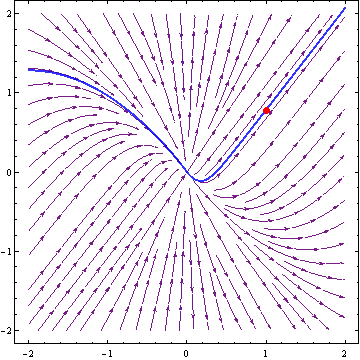
\includegraphics[width=7cm]{images/04_analisis2/tp12_ej1c.png}
\end{center}


\section{Ecuaciones Diferenciales de Variables Separables}

\begin{definition}
Una EDO se dice que es de \textbf{variables separables} \index{Ecuación Diferencial!Variables Separables} si mediante operaciones algebraicas se la puede llevar a la forma

$$ y' = \frac{p(x)}{q(y)} $$

o, usando la notacion de Leibniz

$$ q(y)dy = p(x)dx $$

\end{definition}

Para resolverla, es decir encontrar su SG, basta con integrar ambos miembros (es decir hallar una primitiva), y agregar una constante arbitraria en un lado de la igualdad.

$$ \int q(y)dy = \int p(x)dx + C$$

\section{Ecuación Diferencial Ordinaria Lineal de 1º Orden}

\begin{definition} \label{edo_lineal_orden_n}

Una ecuación diferencial se dice que es una \textbf{ecuación diferencial lineal de orden $n$} \index{Ecuación Diferencial!Lineal} si se puede expresar de la forma

$$ y^{(n)} + a_{n-1}y^{n-1} + \ldots + a_1(x)y' + a_0(x) y = g(x) $$

Si $ g(x) \equiv 0$ es la función constante 0, se dice que la EDO es \textbf{lineal homogénea}. \index{Ecuación Diferencial!Lineal!Homogénea}

\end{definition}

Un caso particular es la ecuación diferencial lineal de 1º orden

\begin{definition}

Una ecuación diferencial se dice \textbf{lineal de 1er orden} \index{Ecuación Diferencial!Lineal!De 1er orden} se puede expresar como

$$ y' + p(x) y = q(x) $$

\end{definition}

\begin{proposition} \label{resolucion_lineal_1er_orden}

Dada la ecuación diferencial lineal de 1º orden

$$ y' + p(x) y = q(x) $$

Su solución general es 

$$ y = e^{-\int p(x) dx} \int q(x) e^{\int p(x) dx} dx + C e^{-\int p(x) dx} $$

\end{proposition}

\begin{proof}

Hay varios métodos de resolución para una EDO lineal de 1º orden.  

Uno fácil es el siguiente: empezamos por realizar la sustitución 

$$ y = uv $$

con lo cual nos queda 

$$ y' = u'v + uv' $$

reemplazamos

$$ u'v + uv' + p(x) uv = q(x) $$

Ahora sacar factor común $v$ (o $u$, la relación es en principio simétrica)

$$ v[u' + p(x) u] + uv' = q(x) $$

Imponemos la condición de que lo que multiplica a $v$ sea cero

$$ u' + p(x) u = 0 $$

Nos queda una EDO en $u$ de variables separables

$$ \int \frac{du}{u} = \int -p(x) dx$$

Buscamos una SP de la misma (no hace falta la constante arbitraria), obtenemos

$$ u = e^{-\int p(x) dx} $$

Ahora reemplazamos la SP de $u$ encontrada en la EDO y nos queda

$$ e^{- \int p(x) dx} v' = q(x) $$

Y nos quedó una EDO en $v$ de variables separables, la resolvemos

$$ \int dv = \int q(x) e^{\int p(x) dx} dx $$

Esta vez queremos la SG de $v$ (por eso va la constante arbitraria)

$$ v = \int q(x) e^{\int p(x) dx} dx + C $$

Finalmente reemplazamos $u$ y $v$ (no olvidar distribuir el paréntesis)

$$ y = uv $$

$$ y = e^{-\int p(x) dx} \int q(x) e^{\int p(x) dx} dx + C e^{-\int p(x) dx} $$

\end{proof}

Como se podrá imaginar, no es sencillo recordar dichar fórmula, es por eso que se aconseja en cambio recordar el método de resolución, es decir recordar sustituir $ y = uv$ y hacer los mismos pasos.

\section{Familias de curvas}

\begin{definition}[Flía de curvas]

Dada una ecuación en la que interviene una variable independiente, una variable dependiente, y $n$ constantes arbitrarias $ c_1, \ldots, c_n \in \RR$, llamamos \textbf{familia de curvas} \index{Ecuación Diferencial!Flía de curvas} (de orden $n$) a las curvas que se obtienen de asignarle valores a las constantes arbitrarias.

Simbólicamente la podemos expresar una familia de curvas de la forma

$$ F(x,y,c_1,\ldots, c_n) = 0 $$

\end{definition}

Cuando encontramos la SG de una EDO $\mathcal{E}$ de orden $n$, la misma viene expresada por una familia de curvas $\mathcal{F}$ de orden $n$.

Las funciones que son solución, quedan expresadas por una ecuación que define a $y$ implícitamente en función de $x$. 

No siempre es posible o conveniente explicitar dichas funciones.

Recíprocamente, dada una familia de curvas $\mathcal{F}$ de orden $n$, podemos buscar una EDO $\mathcal{E}$ de orden $n$ tal que dicha familia sea su SG.

\subsection{Familias de curvas ortogonales}

\begin{definition}[Flía ortogonal]

Sean $C_1$ y $C_2$ en $\RR^2$ dos curvas que se cortan en $A = (x_0, y_0)$, es decir tal que $A \in C_1 \cap C_2$.  Decimos que $C_1$ y $C_2$ son \textbf{curvas ortogonales en $A$} si admiten vector tangente en dicho punto, y los mismos son ortogonales (o equivaléntemente, si admiten rectas tangentes en dicho punto, y las mismas son ortogonales).

Es decir, si $g_1 : [a,b] \to \RR^2$ y $g_2 : [c,d] \to \RR^2$ son parametrizaciones regulares de $C_1$ y $C_2$ respectivamente, tal que $g_1(t_1) = g_2(t_2) = A$, entonces $ g'_1(t_1) \cdot g'_2(t_2) = 0$

Dos familias de curvas $\mathcal{F}_1$ y $\mathcal{F}_2$ se dicen \textbf{familias de curvas ortogonales}, \index{Ecuación Diferencial!Flía de curvas!Ortogonal} si para toda $C_1 \in \mathcal{F}_1$, $C_2 \in \mathcal{F}_2$, resultan ser curvas ortogonales para todo punto de intersección $A \in C_1 \cap C_2$.
\end{definition}

Los siguientes gráficos representan familias de curvas ortogonales.

\begin{center}
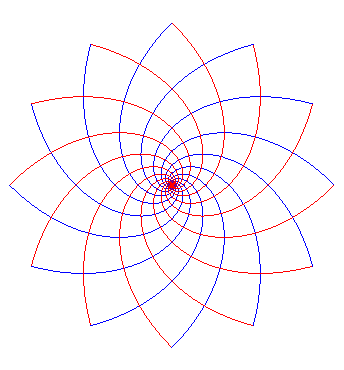
\includegraphics[width=5cm]{images/04_analisis2/flias_ortogonales1.png}
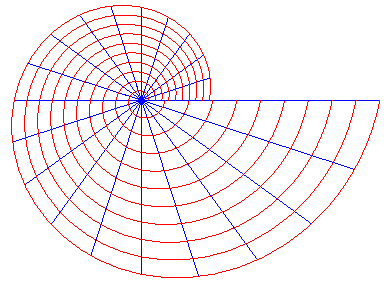
\includegraphics[width=5cm]{images/04_analisis2/flias_ortogonales2.png}

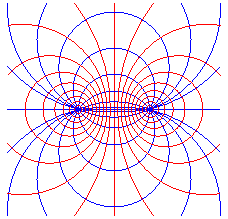
\includegraphics[width=5cm]{images/04_analisis2/flias_ortogonales5.png}
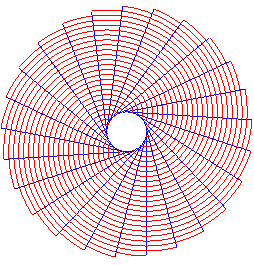
\includegraphics[width=5cm]{images/04_analisis2/flias_ortogonales4.png}

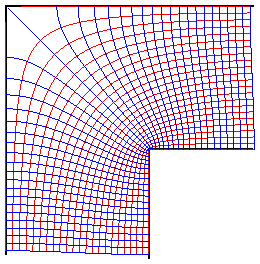
\includegraphics[width=5cm]{images/04_analisis2/flias_ortogonales3.png}
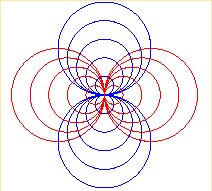
\includegraphics[width=5cm]{images/04_analisis2/flias_ortogonales6.png}
\end{center}

\begin{proposition}

Dos familias de curvas $\mathcal{F}_1, \mathcal{F}_2$ son ortogonales sii sus respectivas ecuaciones diferenciales $\mathcal{E}_1, \mathcal{E}_2$ están relacionadas por la ecuación

$$ y'_2 = \frac{-1}{y'_1}$$

\end{proposition}

\begin{proof} (Enfoque Cartesiano)

Sabemos que si tenemos dos rectas que pasan por $(x_0, y_0)$ de ecuaciones 

$ y_1 - y_0 = m_1 (x-x_0)$

$ y_2 - y_0 = m_2 (x-x_0)$

entonces las mismas son ortogonales sii $m_2 = -1/m_1$.

Sean las curvas $C_1 \in \mathcal{F}_1, C_2 \in \mathcal{F}_2$ de ecuación

$ y_1 = y_1(x)$

$ y_2 = y_2(x)$

Las mismas admiten recta tangente en $(x_0, y_0)$

$ y = y_1(x_0) + \underbrace{m_1}_{y_1'(x_0)} (x-x_0)$ 

$ y = y_2(x_0) + \underbrace{m_2}_{y_2'(x_0)} (x-x_0)$ 

y luego las mismas son ortogonales sii se cumple

$ y_2'(x_0) = - \frac{1}{y_1'(x_0)}$
\end{proof}

\begin{proof} (Enfoque paramétrico)

Dadas las curvas $C_1 \in \mathcal{F}_1, C_2 \in \mathcal{F}_2$ de ecuaciones

$ y = y_1(x)$

$ y = y_2(x)$ 

Las podemos parametrizar como

$ g_1(t) = (t, y_1(t) )$

$ g_2(t) = (t, y_2(t) )$

Luego podemos encontrar vectores tangentes a cada una derivando

$ g_1'(t) = (1, y_1'(t) )$

$ g_2'(t) = (1, y_2'(t) )$

y estos son ortogonales sii su producto escalar es cero

$ g_1'(t) \cdot g_2'(t) = 0$

$ (1,y_1'(t)) \cdot (1, y_2'(t)) = 0$

$ 1 + y_1'(t) y_2'(t) = 0$

Finalmente,

$ y_2'(t) = -\frac{1}{y_1'(t)}$
\end{proof}



% % % % % % % % % % % % % % % % % % % % % % % % % % % % % %

\chapter{Nociones de Topología}

\section{Espacio euclídeo}

\begin{definition} \label{espacio euclideo}
Llamamos \textbf{espacio euclídeo}, \index{Espacio Euclídeo} a un espacio vectorial sobre $\RR$ con un producto interno. 
\end{definition}

\begin{definition} \label{producto escalar}
Definimos el \textbf{producto interno usual de $\RR^n$} (o producto escalar) \index{Espacio Euclídeo!Producto escalar} de la siguiente manera: dados $v,w \in \RR^n$, su producto interno usual es

$$ \vec{v} \cdot \vec{w} = v_1w_1 + v_2w_2 + \ldots + v_nw_n $$
\end{definition}

El espacio euclídeo en el que vamos a trabajar en esta materia es $ \RR^n$ con el producto interno usual.  De ahora en más cada vez que se mencione $\RR^n$ lo vamos a pensar como un espacio euclídeo.

El producto interno nos permite definir las nociones de norma de un vector, distancia entre dos vectores, y ángulo entre dos vectores, como mostramos a continuación

\begin{definition}[Norma]
Dado $v \in \RR^n$, definimos su \textbf{norma} como

$$ ||\vec{v}|| = \sqrt{\vec{v} \cdot \vec{v}} = \sqrt{v_1^2 + v_2^2 + \ldots v_n^2} $$

y dados $v,w \in \RR^n$, definimos su \textbf{distancia} como

$$ d(v, w) = ||w-v|| = \sqrt{ (w_1 - v_1)^2 + (w_2 - v_2)^2 + \ldots + (w_n - v_n)^2 } $$

y su \textbf{ángulo} como

$$ \cos(\phi) = \frac{\vec{v} \cdot \vec{w}}{||\vec{v}|| \ || \vec{w}||} $$
\end{definition}


\section{Entorno}

\begin{definition}[Entorno]
Dados $x \in \RR^n$ y $r > 0$ 

Llamamos \textbf{entorno} \index{Espacio Euclídeo!Entorno} (o entorno abierto) de centro $x_0$ y radio $r$ al conjunto

$$ E(x,r) = \{ y \in \RR^n : d(x,y) < r\} $$

Llamamos \textbf{entorno cerrado} de centro $x_0$ y radio $r$ al conjunto

$$ E[x,r] = \{ y \in \RR^n : d(x,y) \leq r\} $$

Llamamos \textbf{entorno reducido} de centro $x$ y radio $r$ a 

$$ E'(x,r) = E(x,r) - \{x\}$$
\end{definition}

\section{Clasificación topológica de puntos de $\RR^n$}

\begin{definition}[Puntos]

Sea $A \subseteq \RR^n$, y $x \in \RR^n$, entonces decimos que $x$ respecto de $A$ es 

\begin{itemize}
\item \textbf{Punto interior}: Si existe $E(x,\delta) \subseteq A$.

\item \textbf{Punto exterior}: Si existe $E(x,\delta) \subseteq \RR^n - A$.  Equivaléntemente $E(x,\delta) \cap A = \emptyset$.

\item \textbf{Punto frontera}: Si no es punto interior ni exterior.  Es decir que para todo $ \delta > 0$ se tiene $E(x,\delta) \cap A \neq \emptyset$ y $E(x,\delta) \cap (\RR^n - A) \neq \emptyset$

\item \textbf{Punto clausura} (o adherencia): Si existe un entorno tal que $E(x,r) \cap A \neq \emptyset$

\item \textbf{Punto de acumulación} (o punto límite): Si para todo entorno del punto, $ E(x,r) \cap (A - \{x\}) \neq \emptyset$.

Equivaléntemente, si para todo entorno reducido del punto, $ E'(x,r) \cap A \neq \emptyset$

\item \textbf{Punto aislado}: Si existe un entorno tal que $E(x,r) \cap A = \{x\}$
\end{itemize}
\end{definition}

\begin{definition}
Sea $A \subseteq \RR^n$.  Entonces definimos

El \textbf{interior de $A$} como el conjunto de sus puntos interiores, lo denotamos $A^{\circ}$

La \textbf{clausura de $A$} como el conjunto de sus puntos de clausura, lo denotamos $\overline{A}$

El \textbf{conjunto derivado de $A$} como el conjunto de todos sus puntos de acumulación, lo denotamos $A'$

\end{definition}

\begin{observation}

Dado $A \subseteq \RR^n$, se cumple que $ A^{\circ} \subseteq A \subseteq \overline{A}$.

\end{observation}

\section{Clasificación topológica de subconjuntos de $\RR^n$}

\begin{definition}[Abierto]
Sea $A \subseteq \RR^n$, decimos que $A$ es un conjunto

\begin{itemize}
\item Abierto: Si $A=A^{\circ}$. \index{Espacio Euclídeo!Conjunto Abierto} Es decir si todos los puntos del conjunto son interiores.

\item Cerrado: Si $A = \overline{A}$. \index{Espacio Euclídeo!Conjunto Cerrado} Es decir si todos los puntos de clausura pertenecen al conjunto. Equivaléntemente
\begin{itemize}
\item El conjunto contiene a todos sus puntos frontera.
\item El conjunto contiene a todos sus puntos de acumulación.  
\item El complemento del conjunto es abierto.
\end{itemize}
\end{itemize}
\end{definition}

\begin{observation}
Un conjunto puede no ser ni abierto ni cerrado. Por ejemplo $ [0,1) \subset \RR$.

Además un conjunto puede ser abierto y cerrado a la vez. Por ejemplo $ \emptyset$ y $ \RR^n$.
\end{observation}

\section{Conjunto acotado}

\begin{definition}[Acotado]
Un conjunto $A \subseteq \RR^n$ se dice que es un \textbf{conjunto acotado} \index{Espacio Euclídeo!Conjunto Acotado} si el mismo está contenido en algún entorno del origen, es decir si $ A \subseteq E(0, r)$ para algún $r > 0$.
\end{definition}

\section{Conjunto conexo}

Intuitivamente, un conjunto conexo es aquel formado por una sola 'pieza', que no se puede 'dividir'.

\begin{definition}[Conexo]
Una \textbf{escisión} de un conjunto $X \subseteq \RR^n$ son dos conjuntos disjuntos abiertos $A,B$ tales que $ X \subseteq A \cup B$.  Decimos que la misma es no trivial si $A \cap X \neq \emptyset$ y $B \cap X \neq \emptyset$.

Un conjunto $ X \subseteq \RR^n$ es un \textbf{conjunto conexo} \index{Espacio Euclídeo!Conjunto Conexo} si no admite escisiones no triviales.  

En caso contrario decimos que es \textbf{disconexo}.
\end{definition}

\begin{example}
Para ejemplificar esta parte vamos a utilizar estos tres conjuntos

\begin{itemize}
\item $ A = \RR^n $

\item $ B = S^1 = \{ (x,y) \in \RR^2 : x^2 + y^2 = 1\}$

\item $ C = D^2(4,4) = \{ (x,y) \in \RR^2 : (x-4)^2 + (y-4)^2 \leq 1 \}$ 
\end{itemize}

Los tres conjuntos $A$, $B$ y $C$ son conjuntos conexos.

En cambio $D = B \cup C$ es disconexo, pues si $X = E((0,0),2))$ y $Y=E((4,4), 2)$ se tiene $X$ e $Y$ abiertos, y disjuntos, $ D \subseteq X \cup Y$, $X \cap D \neq \emptyset$, $Y \cap D \neq \emptyset$, luego se trata de una escisión no trivial y el conjunto $D$ es disconexo.
\end{example}

\subsection{Conjunto arco-conexo}

\begin{definition}[Camino]
Si $a,b \in \RR^n$, un \textbf{camino} de $a$ a $b$ es una función $ \alpha : [0,1] \to \RR^n$ contínua, tal que $\alpha(0) = a$ y $\alpha(1) = b$
\end{definition}

\begin{example}
Si $a, b \in \RR^n$ el \textbf{camino recto} entre $a$ y $b$ es la función $\alpha : [0,1] \to \RR^n$ tal que

$$ \alpha(t) = ta + (1-t)b $$

La imagen de dicho camino es el segmento de recta

$$ [a,b] = \{ ta + (1-t)b : t \in [0,1] \} $$
\end{example}

\begin{definition}[Arco-conexo]
Un conjunto $A \subseteq \RR^n$ se dice que es un \textbf{conjunto arco-conexo} \index{Espacio Euclídeo!Conjunto Arco-conexo} si para todos los $a,b \in A$ existe un camino $\alpha$ que une $a$ con $b$ dentro del conjunto, es decir tal que $\alpha([0,1]) \subseteq A$.
\end{definition}

\begin{example}
Siguiendo con el ejemplo, los conjuntos $A,B,C$ son todos arco-conexos.
\end{example}

\begin{observation}
Todo conjunto arco-conexo es conexo, pero no vale la vuelta, es decir hay conjuntos conexos que no son arco-conexos.
\end{observation}

\begin{definition}
Si $\alpha$ es un camino de $a$ a $b$, y $\beta$ es un camino de $b$ a $c$, definimos la \textbf{yuxtaposición} de $\alpha$ y $\beta$ como el camino $ \alpha \wedge \beta : [0,1] \to \RR^n$ de $a$ a $c$ definido por 

\[
(\alpha \wedge \beta)(t) = 
\begin{cases}
\alpha(t) &  t \in [0, \frac{1}{2}] \\
\beta(2t-1) &  t \in [\frac{1}{2},1]
\end{cases}
\]
\end{definition}

\subsection{Conjunto conexo por poligonales}

\begin{definition}[Poligonal]
Una \textbf{poligonal} $\pi$ es la yuxtaposición de $k \in \mathbb{N}$ caminos rectos $\pi_i : [x_{i-1}, x_i] \to \RR^n$ con $1 \leq i \leq k$. 
\end{definition}

\begin{definition}
Un conjunto $A \subseteq \RR^n$ se dice que es un \textbf{conjunto conexo por poligonales} si para todo $a, b \in A$ existe una poligonal $\pi$ que comienza en $a$, termina en $b$, y está contenida en $A$.
\end{definition}

\begin{observation}
Una poligonal es un caso particular de un camino.  Por lo tanto si un conjunto es conexo por poligonales, entonces también es arco-conexo, pero no vale la vuelta.
\end{observation}

\begin{example}
En los ejemplos, los conjuntos $A$ y $C$ son conexos por poligonales, aunque el conjunto $B$ (que es arco-conexo) no es conexo por poligonales.
\end{example}

\subsection{Conjunto convexo}

\begin{definition}[Convexo]
Un conjunto $A \subseteq \RR^n$ se dice que es un \textbf{conjunto convexo} \index{Espacio Euclídeo!Conjunto Convexo} si para todo $a, b \in A$ el camino recto que los une no se sale del conjunto, es decir $[a,b] \subseteq A$.
\end{definition}

\begin{observation}
Un camino recto es un caso particular de una poligonal, por lo tanto un conjunto convexo también es conexo por poligonales.
\end{observation}

\subsection{Conjunto símplemente conexo}

Esta es la noción más compleja de conexidad que vemos.  Intuitivamente, un conjunto es símplemente conexo si toda curva cerrada simple (curva de Jordan) se puede "deformar contínuamente" hasta llegar a un punto.  En $ \RR^2$ esto sería equivalente a decir que el conjunto no tiene agüjeros.  

Más formalmente, si denotamos $S^1$ al círculo unitario de $\RR^2$ y $D^2$ al disco unitario de $\RR^2$, es decir

$$ S^1 = \{(x,y) \in \RR^2 : x^2 + y^2 = 1 \} $$

$$ D^2 = \{(x,y) \in \RR^2 : x^2 + y^2 \leq 1 \} $$

entonces se tiene la siguiente

\begin{definition}[Simpl. conexo]
Un conjunto $X$ es un \textbf{conjunto símplemente conexo} \index{Espacio Euclídeo!Conjunto Símplemente Conexo} si es arco-conexo, y además toda función contínua $f : S^1 \to X$ se puede extender a una función contínua $F : D^2 \to X$ tal que $F$ restringida a $S^1$ es $f$, y tal que la imágen de $F$ no se sale del conjunto, es decir $F(D^2) \subseteq X$.
\end{definition}

\section{Clasificación de funciones}

\begin{definition}
Sea $f$ una función de la forma $ f : A \subseteq \RR^n \to \RR^m$.  

Entonces

\begin{itemize}
\item Si $n=m=1$ decimos que $f$ es una \textbf{función escalar}. \index{Espacio Euclídeo!Funciones!Función escalar}

\item Si $n=1$ y $m>1$ decimos que $f$ es una \textbf{función vectorial}. \index{Espacio Euclídeo!Funciones!Función vectorial}

\item Si $n>1$ y $m=1$ decimos que $f$ es un \textbf{campo escalar}. \index{Espacio Euclídeo!Funciones!Campo escalar}

\item Si $n>1$ y $m>1$ decimos que $f$ es un \textbf{campo vectorial}. \index{Espacio Euclídeo!Funciones!Campo vectorial}
\end{itemize}

\end{definition}

Tiene sentido decir que las funciones más generales que estudiamos son los campos vectoriales, y que las otras son casos particulares, y que la función escalar es la que se estudió en Análisis 1.  En esta materia generalizamos a más de una dimensión tanto en el dominio como el codominio de las funciones.

\section{Conjuntos de nivel}

\begin{definition}[Cjto. de nivel]
Sea $f : A \subseteq \RR^n \to \RR$ un campo escalar, y sea $k \in \RR$

El \textbf{conjunto de nivel $k$ de $f$} \index{Espacio Euclídeo!Funciones!Cjto de nivel} es la preimágen de $k$ por $f$, es decir 

$$ C_k(f) = f^{-1}(k) = \{x \in A : f(x) = k \} $$
\end{definition}

Análogamente, podemos definir el conjunto de positividad como sigue

\begin{definition}[Positividad]
Sea $f : A \subseteq \RR^n \to \RR$ un campo escalar.

El \textbf{conjunto de positividad de $f$} es la preimagen del conjunto de todos los reales positivos, es decir

$$ C^+(f) = f^{-1}((0,+\infty)) = \{x \in A : f(x) > 0 \} $$
\end{definition}


% % % % % % % % % % % % % % % % % % % % % % % % % % % % % %

\chapter{Límite y Continuidad}

\begin{definition}[Límite]
Sea $f : A \subset \RR^n \to \RR^m$, $ a \in A'$, y $L \in \RR^n$.  Se dice que existe el \textbf{límite de $f$ cuando $x$ tiende a $a$} \index{Continuidad!Límite} es $L$ si se cumple cualquiera de las siguientes afirmaciones equivalentes

\begin{enumerate} 

\item Para todo $\epsilon > 0$ existe $\delta > 0$ tal que si $x \in A$, $0 < ||x-a|| < \delta$ entonces $||f(x) - L|| < \epsilon$

\item Para todo $\epsilon > 0$ existe $\delta > 0$ tal que si $x \in E^*(a,\delta) \cap A$ entonces $f(x) \in E(L,\epsilon)$

\item Para todo $\epsilon > 0$ existe $\delta > 0$ tal que $f(E^*(a,\delta) \cap A) \subseteq E(L,\epsilon)$

\item Para todo $\epsilon > 0$ existe $\delta > 0$ tal que $E^*(a,\delta) \cap A \subseteq f^{-1}(E(L,\epsilon))$

\end{enumerate}

y en ese caso lo denotamos escribiendo

$$ \displaystyle \lim_{x \to a} f(x) = L $$

\end{definition}


\begin{definition}[Continuidad]
Sea $ f: A \subset \RR^n \to \RR^m$, y sea $a \in A$.  Se dice que $f$ es \textbf{contínua en $a$} \index{Continuidad} si se cumple cualquiera de las siguientes afirmaciones equivalentes

\begin{enumerate} 
\item Para todo $\epsilon > 0$ existe $\delta > 0$ tal que si $x \in A$, $||x-a|| < \delta$ entonces $||f(x) - f(a)|| < \epsilon$

\item Para todo $\epsilon > 0$ existe $\delta > 0$ tal que si $x \in E(a,\delta) \cap A$ entonces $f(x) \in E(f(a),\epsilon)$

\item Para todo $\epsilon > 0$ existe $\delta > 0$ tal que $f(E(a,\delta) \cap A) \subseteq E(f(a),\epsilon)$

\item Para todo $\epsilon > 0$ existe $\delta > 0$ tal que $E(a,\delta) \cap A \subseteq f^{-1}(E(f(a),\epsilon))$
\end{enumerate}
\end{definition}

La relación entre los conceptos de límite y continuidad viene dada por la siguiente

\begin{observation}
Si $a \in A$ es punto aislado de $A$, entonces $f$ es contínua en $a$ (basta tomar el $\delta$ que hace que el punto sea aislado).

De lo contrario, $a \in A$ es un punto de acumulación de $A$, en este caso $f$ es contínua en $a$ sii se cumplen las siguientes

\begin{enumerate}
\item Existe $f(a)$ (en realidad esto ya lo estamos pidiendo cuando decimos $a \in A$)

\item Existe $\displaystyle \lim_{x \to a} f(x) = L$ 

\item $f(a) = L$
\end{enumerate}
\end{observation}

Para analizar la continuidad de una función compuesta resulta muy útil el siguiente 

\begin{theorem}
Si $f : A \subseteq \RR^n \to B \subseteq \RR^m$ es contínua en $a$ y $ g : B \subseteq \RR^m \to \RR^p$ es contínua en $b = f(a)$, y si llamo $h = g \circ f$, entonces $h$ es contínua en $a$.
\end{theorem}

\begin{proof}[Demostración (Optativa)]
Como $g$ es contínua en $b = f(a) \in B$ entonces dado $\epsilon > 0$ existe $\delta_g > 0$ tal que si $y \in B$, $||y - f(a)|| < \delta_g$ entonces $||g(y) - g(f(a))|| < \epsilon$.

Como $f$ es contínua en $a \in A$, existe $\delta_f$ tal que si $x \in A$, $||x-a|| < \delta_f$ entonces $||f(x) - f(a)|| < \delta_g$

Luego, si $x \in A$, $||x-a|| < \delta_f$ entonces $||f(x) - f(a)|| < \delta_g $ entonces $||g(f(x)) - g(f(a))|| < \epsilon$
\end{proof}

Para analizar la continuidad de una función vectorial o de un campo vectorial, suele ser útil la siguiente

\begin{observation}
Si $f : A \subseteq \RR^n \to \RR^m$ tiene funciones coordenadas $f = (f_1, f_2, \ldots, f_m)$ entonces $f$ es contínua en $a$ si y solo sí cada componente $f_i$ es contínua en $a$ para todo $1 \leq i \leq m$.
\end{observation}

\begin{proof}[Demostración (Optativa)]
$\Rightarrow$) Suponemos $f$ contínua en $a$. Considero la proyección $P_j : \RR^m \to \RR$ tal que $P_j(x_1, \ldots, x_m) = x_j$.  Es Lipschitziana, pues $|x_j - y_j| \leq 1 \cdot || \vec{x} - \vec{y} ||$.

Luego $f_j = P_j \circ f$ es contínua en $a$ por ser composición de contínuas.

$\Leftarrow$) Suponemos $f_1, \ldots, f_m$ contínuas en $a$

Es decir, dado $\epsilon > 0$ existe $\delta > 0$ tal que $||x-a|| < \delta \Rightarrow |f_j(x) - f_j(a)| < \frac{\epsilon}{m}$

Luego $|| f(x) - f(a) || \leq \sum_{j=1}^m |f_j(x) - f_j(a)| < \sum_{j=1}^m \frac{\epsilon}{m} \leq \epsilon$.
\end{proof}

Ojo con esto:

\begin{observation}
Si una función de varias variables es contínua en cada variable por separado, no es suficiente para asegurar la continuidad de la función.
\end{observation}

\begin{proof}
Sea por ejemplo $f: \RR^2 \to \RR$ definida por

$$f(x,y) = \begin{cases} 
\frac{y}{x} - y & 0 \leq y < x \leq 1 \\ 
\frac{x}{y} - x & 0 \leq x < y \leq 1 \\ 
1-x & 0 \leq x = y \leq 1 \\ 
0 & \forall \textrm{ otro } (x,y)  
\end{cases}$$

Se puede chequear que todas las funciones reales $f_y(x) = f(x,y)$ son contínuas para todo $x$ (para $y$ fijado).

Similarmente, es fácil ver que $f_x$ es contínua para todo $y$ ($x$ fijado)

Sin embargo $f$ no es contínua, ya que en el origen $f(0,0) = 0$, pero $\lim_{n \to \infty} f(\frac{1}{n}, \frac{1}{n}) = 1 \neq 0$

A continuación se muestra la gráfica de $f$ en el cuadrado $[0,1] \times [0,1]$ (fuera de allí la función vale 0).

\begin{center}
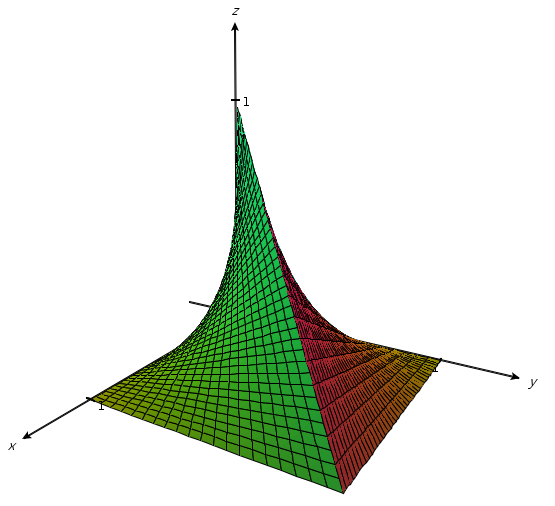
\includegraphics[width=5cm]{images/04_analisis2/func_discontinua1.png}

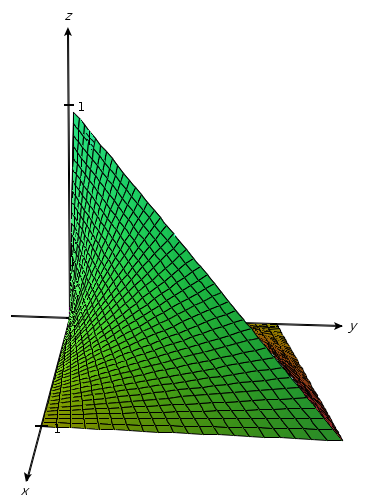
\includegraphics[width=5cm]{images/04_analisis2/func_discontinua2.png}
\end{center}

Se ve que al analizar la continuidad en el origen por los ejes $x$ e $y$ el límite existe y da cero, mientras que por la semirecta $y=x$ con $x >0$ el límite da 1.
\end{proof}

Y ojo también con esto:

\begin{observation}
Supongamos que tenemos $f: A \subseteq \RR^n \to B \subseteq \RR^m$, $g : B \subseteq \RR^m \to \RR^p$ y $h = g \circ f$, tales que $\lim_{x \to a} f(x) = L_f$ y $\lim_{y \to L_f} g(y) = L_g$.  Todo ello no implica que $\lim_{x \to a} h(x) = L_g$
\end{observation}

\begin{proof}
Damos un contraejemplo:  Si $f(x) = L_f$ y $g(y) = \begin{cases} L_{g1} & y = L_f \\ L_{g2} & y \neq L_f \end{cases}$, entonces

$\lim_{x \to a} f(x) = L_f$ y $\lim_{y \to L_f} g(y) = L_{g2}$, pero $h(x) = g(f(x)) = L_{g1}$, luego no es cierto que $\lim_{x \to a} h(x) = L_{g2}$.
\end{proof}

Lo que si es cierto la siguiente

\begin{observation}[Optativa] \label{limite_compuesta_1}
Dados $f: A \subseteq \RR^n \to B \subseteq \RR^m$, $g : B \subseteq \RR^m \to \RR^p$, y $h = g \circ f$, tales $\lim_{x \to a} f(x) = L$, y que $g$ es contínua en $L$, con $c = g(L)$ entonces $\lim_{x \to a} h(x) = c$
\end{observation}

\begin{proof}
Como $g$ es contínua en $L \in B$ entonces dado $\epsilon > 0$ existe $\delta_g > 0$ tal que si $y \in B$, $||y - L|| < \delta_g$ entonces $||g(y) - g(L)|| < \epsilon$.

Como $\lim_{x \to a} f(x) = L$, existe $\delta_f$ tal que si $x \in A$, $0 < ||x-a|| < \delta_f$ entonces $||f(x) - L|| < \delta_g$

Luego, si $x \in A$, $0 < ||x-a|| < \delta_f$ entonces $||f(x) - L|| < \delta_g $ entonces $||g(f(x)) - g(L)|| < \epsilon$
\end{proof}

\begin{example}
Calcular $\lim_{(x,y) \to (1,1)} (\frac{x^2 - y^2}{x-y})^2 + 3 $.

Si llamamos $f(x,y) = \frac{x^2 - y^2}{x-y}$, $g(z) = z^2 + 3$ y $h = g \circ f$, nos piden $\lim_{(x,y) \to (1,1)} h(x,y)$.

Como $f(x,y) = \frac{x^2 - y^2}{x-y} = \frac{(x-y)(x+y)}{x-y} = x+y$, se tiene $\lim_{(x,y) \to (1,1)} f(x,y) = 1+1 = 2 $, pero notar que $f$ no está definida en $(1,1)$ luego no es contínua en él.

Como $g$ es contínua en $2$ y $g(2) = 2^2 + 3 = 7$, por la observación \ref{limite_compuesta_1} se tiene que $\lim_{(x,y) \to (0,0)} h(x,y) = 7$
\end{example}

Esta misma conclusión sobre el límite de la compuesta se puede alcanzar sin pedir $g$ contínua en el punto, pero con otra hipótesis, es decir:

\begin{observation}[Optativa] \label{limite_compuesta_2}
Dados $f: A \subseteq \RR^n \to B \subseteq \RR^m$, $g : B \subseteq \RR^m \to \RR^p$, y $h = g \circ f$, tales $\lim_{x \to a} f(x) = L_f$, y $\lim_{y \to L_f} g(y) = L_g$, y si además para todo $\epsilon > 0$ existe $\delta > 0$ tal que si $x \in A$, $0 < ||x-a|| < \delta$ luego $0 < || f(x) - L_f|| < \epsilon$, pues entonces $\lim_{x \to a} h(x) = L_g$
\end{observation}

\begin{proof}
Como $\lim_{y \to L_f} g(y) = L_g$, para todo $\epsilon > 0$ existe $\delta_g > 0$ tal que si $y \in B$, $0 < |y-L_f| < \delta_g$ entonces $|g(y) - L_g| < \epsilon$

Como $\lim_{x \to a} f(x) = L_f$, para todo $\delta_g > 0$ existe $\delta_f > 0$ tal que si $x \in A$, $0 < |x-a| < \delta_f$ entonces $|f(x) - L_f| < \delta_g$.

Pero por la hipótesis extra, también existe $\delta'_f > 0$ tal que si $x \in A$, $0 < ||x-a|| < \delta'_f$ luego $0 < || f(x) - L_f|| < \delta_g$.

Finalmente, $x \in A$, $0 < ||x-a|| < \delta'_f$ implica $0 < || f(x) - L_f|| < \delta_g$ que implica $|g(y) - L_g| < \epsilon$, es decir que $\lim_{x \to a} h(x) = L_g$.
\end{proof}

\begin{example}
Calcular $\lim_{(x,y) \to (0,0)} \frac{\sin(x^2 + y^2)}{x^2 + y^2}$.

Si llamamos $f(x,y) = x^2 + y^2$, $g(z) = \frac{\sin(z)}{z}$, y $h = g \circ f$, entonces nos piden calcular $\lim_{(x,y) \to (0,0)} h(x,y)$

Sabemos que $\lim_{(x,y) \to (0,0)} f(x,y) = 0$ y que $\lim_{z \to 0} g(z) = 1$.  Como además para todo $\epsilon > 0$ existe $\delta > 0$ tal que si $0 < ||(x,y) - (0,0)|| < \delta$ entonces $ 0 < || f(x,y) - 0 || < \epsilon$, (pues $f(x,y) = 0$ sii $(x,y) = (0,0)$ y $f$ es contínua en $(0,0)$), luego por la observación \ref{limite_compuesta_2} se sigue que $\lim_{x \to a} h(x,y) = 1$
\end{example}

Y también puede ser útil para calcular límites de campos vectoriales el siguiente

\begin{theorem}
Sea $f:A \subseteq \RR^n \to \RR^m$ con funciones coordenadas $ f = (f_1, \ldots, f_m)$ y $a \in A'$, entonces el límite $ \lim_{x \to a} f(x) = L$ existe si y sólo si existen todos los límites $ \lim_{x \to a} f_i(x) = L_i$ con $ 1 \leq i \leq m$, y en dicho caso se tiene $ L = (L_1, \ldots, L_m)$
\end{theorem}

\begin{proof}
$\Rightarrow$) Suponemos $\lim_{x \to a} f(a) = L$. Luego para todo $\epsilon > 0$ existe un $\delta > 0$ tal que para $x \in A$ tal que $0 < ||x-a|| < \delta$ se tiene que $||f(x) - L|| < \epsilon$.  Es decir $\sqrt{ (f_1(x) - L_1)^2 + \ldots + (f_m(x) - L_m)^2} < \epsilon$.  Pero entonces $ \sqrt{ (f_i(x) - L_i)^2 } \leq \sqrt{ (f_1(x) - L_1)^2 + \ldots + (f_m(x) - L_m)^2} < \epsilon$ es decir $|f_i(x) - L_i| < \epsilon$ para todo $1 \leq i \leq m$.  Esto nos dice que $\lim_{x \to a} f_i(x) = L_i$.

$\Leftarrow$) Suponemos $ \lim_{x \to a} f_i(x) = L_i$ para $1 \leq i \leq m$

Es decir, dado $\epsilon > 0$ existe $\delta > 0$ tal que para $x \in A$ con $0 < ||x-a|| < \delta$ se tiene que $|f_j(x) - L_i| < \frac{\epsilon}{m}$

Luego $|| f(x) - L || \leq \sum_{j=1}^m |f_j(x) - L_i| < \sum_{j=1}^m \frac{\epsilon}{m} \leq \epsilon$.
\end{proof}

\begin{proposition}[Propiedades del límite]

Supongamos que las funciones $f, g : A \subseteq \RR^n \to \RR^m$ tales que existen $\lim_{x \to a} f(x) = L_1$ y $\lim_{x \to a} g(x) = L_2$.

Entonces si $h = f \pm g$, se tiene que $ \lim_{x \to a} h(x) = L_1 \pm L_2$.

Y si además $m=1$, es decir se trata de campos escalares, tiene sentido multiplicarlos, y para $h = f \cdot g$ existe $ \lim_{x \to a} h(x) = L_1 \cdot L_2$.

Y también tiene sentido dividirlos en los puntos donde no se anula el denominador, y si $h = f/g$ y $L_2 \neq 0$ entonces $\lim_{x \to a} h(x) = L_1/L_2$.
\end{proposition}

\begin{proposition}[Propiedades de funciones contínuas]

Las siguientes funciones son contínuas en todo su dominio

\begin{itemize}
\item Funciones polinómicas, de cualquier cantidad de variables.
Ejemplo: $x^2 + 3xy + z^3$ es una función contínua en $\RR^3$

\item La función exponencial $f(x) = e^x$ es contínua en $\RR$

\item Las funciones trigonométricas $\sin(x)$ y $\cos(x)$ son contínuas en $\RR$
\end{itemize}

Supongamos que las funciones $f, g : A \subseteq \RR^n \to \RR^m$ son contínuas en $a \in A$. 

Entonces $h = f \pm g$ es contínua en $a$

Y si además $m=1$, es decir se trata de campos escalares, tiene sentido multiplicarlos, y $h = f \cdot g$ es contínua en $a$.

Y también tiene sentido dividirlos en los puntos donde no se anula el denominador, y si $g(a) \neq 0$ entonces $h = f/g$ es contínua en $a$
\end{proposition}

Definamos que es un camino que pasa por $a$ (o que se aproxima a $a$) y que es una vecindad de $a$

\begin{definition}
Sea $A \subseteq \RR^n$ y sea $a \in A'$.  Un \textbf{camino que pasa por $a$} (o que se aproxima a $a$) es un subconjunto $B \subseteq A$ tal que $a \in B'$ (es decir tal que el punto $a$ es punto de acumulación también de $B$).

Un camino $B$ que pasa por $a$ se dice que es una \textbf{vecindad de $a$} si existe $E(a,\delta) = E$ tal que $E \cap A \subseteq B$.
\end{definition}

\begin{example}
Por ejemplo, dado $A \subseteq \RR^n$ y $a \in A'$ y $E = (a, \delta) = E$.  Entonces $B = E \cap A$ es una vecindad de $a$.
\end{example}

Para establecer la existencia y calcular un límite puede ser útil la siguiente observación

\begin{observation}\label{camino_vecindad}
Sea $f: A \subseteq \RR^n \to \RR^m$, $a \in A'$, $B$ una vecindad de $a$, y $g = f|_B$.  Entonces $\lim_{x \to a} f(x) = \lim_{x \to a} g(x)$.  Es decir el límite de $f$ existe sii existe el límite de $g$, y en ese caso son iguales.
\end{observation}

\section{Como probar que un límite no existe}

Si en vez de una vecindad de $a$ tomamos un camino $B \subseteq A$ cualquiera que pasa por $a$, no es cierto que si existe el límite de $g = f|_B$ entonces exista el límite de $f$.  Pero al menos la siguiente proposición nos da un criterio muy útil para probar la no existencia de un límite.

\begin{proposition}
Sea $ f : A \in \RR^n \to \RR$, y $B \subseteq A$ un camino que pasa por $a$ y $g = f|_B$.  Si existe el límite $ \lim_{x \to a} f(x) = L$, entonces también existe el límite $ \lim_{x \to a} g(x) = L$ y son iguales.
\end{proposition}

Esto nos da un criterio para determinar cuando un límite no existe: podemos probar por distintos caminos que pasan por $a$, y si por alguno de ellos el límite no existe, o por dos de ellos existen pero dan valores distintos, entonces el límite de la función $f$ no existe, ya que de otra forma debería existir y ser iguales.

Ojo, aunque pruebe por 727 caminos y todos coincidan en el límite, esto no alcanza para asegurar que el límite de la función original exista, a no ser (por la observación \ref{camino_vecindad}) que por camino tome una vecindad de $a$.

Por lo tanto este criterio sirve para probar que un límite no existe, pero no sirve para probar que un límite exista.

Otra herramienta para determinar cuando un límite no existe son los \textbf{límites laterales}: si estos no coinciden el límite de la función original no existe.

\begin{example}
Sea $ f(x,y) = \frac{ \sin(x^2 + y^4) }{ x^2 + y^2 }$.  Analizar la existencia de límite de $ f$ en $ (0,0)$.

$ \lim_{x \to 0} \left[ \lim_{y \to 0} \frac{ \sin(x^2 + y^4) }{ x^2 + y^2 } \right]$

$ = \lim_{x \to 0} \frac{ \sin(x^2)  }{ x^2 } = 1 = L_{yx}$

$ \lim_{y \to 0} \left[ \lim_{x \to 0} \frac{ \sin(x^2 + y^4) }{ x^2 + y^2 } \right]$

$ = \lim_{y \to 0} \frac{ \sin(y^4) }{ y^2 } $

$ = \lim_{y \to 0} \frac{ 4y^3 \cos(y^4) }{ 2y } $

$ = \lim_{y \to 0} \frac{ 4y^2 \cos(y^4) }{ 2 } = 0 = L_{xy}$

Como $L_{yx} \neq L_{xy}$ no existe el límite pedido.
\end{example}

\section{Como probar que un límite existe}

Una forma que funciona a veces es utilizar el siguiente teorema, familiar desde Análisis 1

\begin{proposition}
Sean $f,g,h:A \subseteq \RR^n \to \RR$, y $a \in A'$.

Si $h = f \cdot g$ con $f$ acotada, es decir $f(A)$ un conjunto acotado, y $g$ infinitésimo, es decir $ \lim_{x \to a} g(x) = 0$ entonces el límite de $h$ cuando $x \to a$ existe y es cero, es decir $ \lim_{x \to a} h(x) = 0$
\end{proposition}

Otra técnica que puede servir es la de relizar un cambio de varibles que reduzca la cantidad de variables.  Por ejemplo, si $f(x,y) = \frac{\sin(x^2 + y^2)}{x^2 + y^2}$, entonces el $ \lim_{(x,y) \to (0,0) } f(x,y) = 0$, pues realizando la sustitución $ u = x^2 + y^2$ se tiene que cuando $(x,y) \to (0,0)$ entonces $u \to 0$ (pues $x^2 + y^2$ es contínua), y por lo tanto el límite pedido equivale a $ \lim_{u \to 0} \frac{\sin(u)}{u} = 1$

% % % % % % % % % % % % % % % % % % % % % % % % % % % % % %

\chapter{Derivabilidad}

\section{Derivada de función vectorial}

\begin{definition}[Derivada]
Dada la función vectorial $ f: A \subset \RR \to \RR^n$ y $ t_0 \in A^{\circ}$, entonces la \textbf{derivada de $f$ en $t_0$} \index{Derivada!de función vectorial} se define como

$$ \displaystyle f'(t_0) = \lim_{h \to 0} \frac{f(t_0 + h) - f(t_0)}{h} $$

si dicho límite existe.  Sinó, se dice que $f$ no es derivable en dicho punto.
\end{definition}

Si es derivable en todo el dominio tiene sentido definir la función derivada $ f'(t)$ que a cada punto $t_0$ le asigna la derivada de la función $f$.  Cuando decimos que $f$ es derivable, sin aclarar el punto, nos referimos a que es derivable en todo su dominio.

Para calcular la derivada suele ser útil la siguiente

\begin{observation}
Si $ f(t) = (f_1(t), f_2(t), \ldots, f_n(t))$ entonces $f$ es derivable si y sólo si todas sus funciones coordenadas $ f_i$ son derivables, y en ese caso el valor de la derivada viene dada por $ g'(t) = (g_1'(t), g_2'(t), \ldots, g_n'(t))$
\end{observation}

\subsection{Interpretación geométrica}
Si $f : [a,b] \to \RR^n$ es la parametrización de una curva $C$, y si además $f$ es derivable en $t_0$, entonces $f'(t_0)$ es un vector tangente a dicha curva en el punto $f(t_0)$.  

\begin{center}
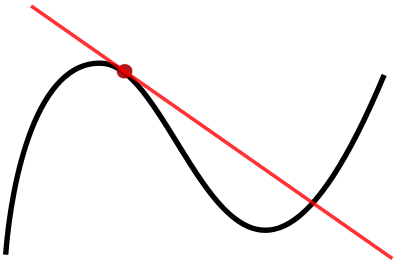
\includegraphics[width=7cm]{images/04_analisis2/tangent.png}
\end{center}

En este caso tiene sentido la siguiente

\begin{definition}
Sea $f : [a,b] \to \RR^n$ parametrización de una curva $C$, y derivable en $t_0$.  Entonces la \textbf{recta tangente a $C$ en $x_0 = f(t_0)$} es de ecuación paramétrica

$$ x = f(t_0) + \lambda f'(t_0) $$

con $\lambda \in \RR$.

Además el \textbf{plano normal a $C$ en $x_0$} es de ecuación cartesiana

$$ (x - f(x_0)) \cdot f'(t_0) = 0 $$
\end{definition}

\section{Derivadas parciales, direccionales, y respecto a un vector}

\begin{definition}
Sea $f : A \subseteq \RR^n \to \RR^m$ y $x_0 \in A^{\circ}$, y sea $v \in \RR^n$.  Entonces definimos la \textbf{derivada de $f$ en $x_0$ respecto al vector $v$} como

$$ \displaystyle f'_v(x_0) = \lim_{h \to 0} \frac{f(x_0 + hv) - f(x_0)}{h} $$

si dicho límite existe.

Si además $v$ es un versor, es decir si $||v|| = 1$, decimos que dicho límite es la \textbf{derivada direccional de $f$ respecto a la dirección $v$}. \index{Derivada!Direccional}

Si además $v$ es un versor canónico de $\RR^n$, es decir si 

$v = e_i = \delta_{ij} = \begin{cases} 1 & i=j \\ 0 & i \neq j \end{cases}$, 

decimos que dicho límite es la \textbf{derivada parcial de $f$ respecto a $x_i$} \index{Derivada!Parcial}

Otras notaciones equivalente son

$ f'_v(x_0) = f'(x_0, v) = D_vf(x_0) = \frac{ \partial f}{\partial v} (x_0)$
\end{definition}

\begin{example}
Dada $f(x,y) = \sqrt{3 - x^2 - y^2} $.  Calculemos las derivadas parciales de $f$ en $(1,0)$

Cuando queremos hacer una derivada parcial, y pensamos las demás variables como constantes, si podemos aplicar la regla de la cadena de Análisis 1 (verificar hipótesis), decimos que estamos aplicando la \textbf{regla práctica}.  En este caso

$$ f'_x(x,y) = \frac{ -2x }{2 \sqrt{3 - x^2 - y^2}} $$

$$ f'_y(x,y) = \frac{-2y }{2 \sqrt{3 - x^2 - y^2}} $$

Luego

$$ f'_x(1,0) = \frac{- 1 }{ \sqrt{3 - 1}} = \frac{-1}{\sqrt{2}} $$

$$ f'_y(1,0) = \frac{- 0 }{ \sqrt{3 - 1}} = 0 $$

Podemos interpretar la derivadas direccional respecto a $v$ como la pendiente de una recta tangente a la gráfica de $z = f(x,y)$ en la dirección de $v$.  

En el siguiente gráfico se representa la gráfica de $z = f(x,y)$, y su recta tangente en $(1,0,f(1,0))$ en la dirección de $y$.  Vemos que la recta resulta ser horizontal, lo que concuerda con que $f'_y(1,0) = 0$ es decir que tiene pendiente nula.

\begin{center}
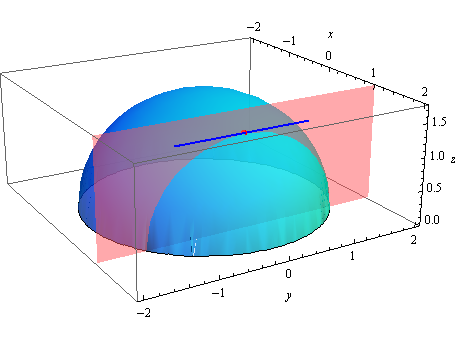
\includegraphics[width=7cm]{images/04_analisis2/tp4_ej5.png}
\end{center}
\end{example}


\begin{definition}
Dada $f : A \subseteq \RR^n \to \RR^m$, 

Decimos que \textbf{$f$ es derivable respecto a $v \in \RR^n$}, sin aclarar el punto, si lo es para todo $x \in \RR^n$.

Decimos que \textbf{$f$ es derivable en $x_0 \in A^{\circ}$}, sin aclarar el vector, si lo es respecto a todo $v \in \RR^n$.

Decimos que \textbf{$f$ es derivable}, sin aclarar ni el punto ni el vector, si lo es para todo $x \in A^{\circ}$ y respecto a todo $v \in \RR^n$.
\end{definition}

El siguiente teorema es útil para derivar funciones vectoriales o campos vectoriales coordenada a coordenada.

\begin{theorem}
Sea $f: A \subseteq \RR^n \to \RR^m$ con $x_0 \in A^{\circ}$ y $v \in \RR^n$, tal que $f = (f_1, \ldots, f_m)$.  Entonces $f$ es derivable en $x_0$ respecto a $v$ si y sólo sí cada función coordenada es derivable en $x_0$ respecto a $v$, y en dicho caso se tiene $f'_v(x_0) = (f'_{1v}(x_0), f'_{2v}(x_0), \ldots, f'_{mv}(x_0))$.
 \end{theorem}

\subsection{Propiedad de homogeneidad}

Llamamos propiedad de homogeneidad de la derivada a la siguiente proposición

\begin{proposition}[Homogeneidad] \index{Derivada!Prop. homogeneidad}
Si existe la derivada direccional $ f'(x_0, v)$ y $ k \in \RR$, $ k \neq 0$, entonces 

$$ f'(x_0, kv) = k f'(x_0, v)$$
\end{proposition}

\begin{proof}
Por definición

$$ \displaystyle f'(x_0, kv) = \lim_{h \to 0} \frac{f(x_0 + hkv) - f(x_0)}{h} $$

multiplico y divido por $k \neq 0$

$$ \displaystyle = k \lim_{h \to 0} \frac{f(x_0 + hkv) - f(x_0)}{hk} $$

Sustituyo $ u = hk$ y cuando $ h \to 0$ se tiene que $ u \to 0$, luego

$$ \displaystyle = k \lim_{u \to 0} \frac{f(x_0 + uv) - f(x_0)}{u} $$

Finalmente

$$ \displaystyle = k f'(x_0, v) $$
\end{proof}

De la propiedad de homogeneidad se desprende fácilmente el siguiente

\begin{corollary}
Sea $f$ derivable en $x_0$, entonces
\begin{itemize}
\item $ f'(x_0, -v) = -f'(x_0, v)$
\item $ f'(x_0, v) = ||v||f'(x_0, \hat{v})$ (donde $ \hat{v} = \frac{v}{||v||}$)
\end{itemize}
\end{corollary}

\begin{proof}
Para el primero basta tomar $k = -1$.  Para el segundo $k = ||v||$.
\end{proof}

\subsection{Derivadas parciales sucesivas}

\begin{definition}
Sea $f: A \subseteq \RR^n \to \RR^m$.  Supongamos esta función es derivable respecto a $x_i$, entonces podemos definir la función derivada parcial $f'_{x_i} : A \to \RR^n$.  Supongamos ahora que esta nueva función es derivable  respecto a $x_j$.  Podemos definir entonces la función derivada segunda parcial

$$ f''_{x_i x_j} : A \to \RR^m $$

A la misma también la llamamos la \textbf{derivada sucesiva respecto a $x_i x_j$}.

Análogamente, si $f$ es $k$ veces derivable, podemos definir la función \textbf{derivada sucesiva respecto a $x_{i_1} x_{i_2} \ldots x_{i_k}$}

$$ f^{(k)}_{x_{i_1} x_{i_2} \ldots x_{i_k}} : A \to \RR^m $$

Si están definidas las funciones derivadas sucesivas $f''_{x_i x_j}$ y $f''_{x_j x_i}$, decimos que estas son \textbf{derivadas sucesivas mixtas}.

Análogamente, si $f$ es $k$ veces derivable, y $\phi : \{1,2, \ldots, k\} \to \{1, 2, \ldots, k\}$ es una permutación, decimos que $f^{(k)}_{x_{i_1} x_{i_2} \ldots x_{i_k}}$ y $f^{(k)}_{x_{i_{\phi(1)}} x_{i_{\phi(2)}} \ldots x_{i_{\phi(k)}}}$ son \textbf{derivadas sucesivas mixtas de orden $k$}.
\end{definition}

\subsection{Teorema de Schwarz}

En palabras sencillas, lo que dice el teorema de Schwarz es que bajo ciertas condiciones, no importa en que orden derivemos va a dar lo mismo.  Es decir que bajo esas condiciones nos garantiza que las derivadas sucesivas mixtas son iguales.

\begin{theorem}[Schwarz] \label{schwarz} \index{Derivada!Teo. Schwarz}
Sea el campo escalar $ f : A \subset \RR^n \to \RR$, si existen $ f''_{x_i x_j}, f''_{x_j x_i}$ y son contínuas en un entorno del punto $ x_0 \in A^{\circ}$ entonces 

$$ f''_{x_i x_j}(x_0) = f''_{x_j x_i}(x_0) $$

es decir las derivadas sucesivas mixtas son iguales.
\end{theorem}

No es fácil encontrar ejemplos de funciones cuyas derivadas sucesivas mixtas no sean iguales.

En 1873 el matemático H.A. Schwarz produjo el siguiente ejemplo

$$ f(x,y) = \begin{cases} x^2 \arctan(y/x) - y^2 \arctan(x/y) & x \neq 0, y \neq 0 \\ 0 & \textrm{en otro caso} \end{cases} $$

Para esta función en $(0,0)$ se tiene que

$$ f''_{xy}(0,0) = -1 \neq f''_{yx}(0,0) = +1 $$

\subsection{Función clase $C^1$}

\begin{definition}[$C^k$]
Si $ f : A \subset \RR^n \to \RR^m$ con $A$ abierto, es tal que posee todas sus derivadas parciales y son contínuas en $ A$, entonces decimos que \textbf{$f$ es de clase $ C^1$} y lo denotamos 

$$ f \in C^1 $$

Del mismo modo si tiene todas sus derivadas parciales segundas y son contínuas decimos que $ f \in C^2$.

Análogamente se dice que $f \in C^k$ si sus derivadas parciales de orden $k$ existen y son contínuas en el abierto $A$. \index{Derivada!Clase $C^k$}
\end{definition}

\begin{observation}
Si $f : A \subset \RR^n \to \RR$, $f \in C^2$, para cualquier $x \in A$ se cumplen las hipótesis del teorema \ref{schwarz} (de Schwarz), es decir  $ f''_{x_i x_j}(x) = f''_{x_j x_i}(x)$.

Más generalmente, si $f \in C^k$, y $\phi : \{1,2, \ldots, k\} \to \{1, 2, \ldots, k\}$ es una permutación, entonces 

$$f^{(k)}_{x_{i_1} x_{i_2} \ldots x_{i_k}} = f^{(k)}_{x_{i_{\phi(1)}} x_{i_{\phi(2)}} \ldots x_{i_{\phi(k)}}}$$

Es decir las \textbf{derivadas sucesivas mixtas de orden $k$} son iguales.
\end{observation}

\section{Curvas y Superficies}

\begin{definition}
Un subconjunto $C \subseteq \RR^n$ decimos que es una \textbf{curva} \index{Curva} si existe una función vectorial contínua $g: [0,1] \to \RR^n$, tal que $ g([0,1]) = C$.  A la función $ g$ se la llama parametrización de la curva.

Sea $ g(t)$ la parametrización de una curva, si además $ g \in C^1$ y existe $ g'(t_0) \neq \vec{0}$ decimos que $x_0 = g(t_0)$ es un \textbf{punto regular de la curva} \index{Curva!Punto regular} $C$.  Si todos los puntos $x_0 \in C$ de la curva son puntos regulares, decimos que $C$ es una \textbf{curva regular}.

Un subconjunto $ \Sigma$ de $ \RR^3$ decimos que es una \textbf{superficie} \index{Superficie} si existe un campo vectorial contínuo $ g: A \subset \RR^2 \to \RR^3$, con $A$ conexo, tal que $ g(A) = S$.  A la función $g$ se le dice la parametrización de la superficie $\Sigma$.

Sea $ g(u,v)$ la parametrización de una superficie, si además $ g \in C^1$ y existe $ g'_u(u_0, v_0) \wedge g'_v(u_0,v_0) \neq 0$ decimos que $x_0 = g(u_0, v_0)$ es un \textbf{punto regular de la superficie} \index{Superficie!Punto regular} $\Sigma$.  Si todos los puntos $x_0 \in \Sigma$ de la superficie son regulares, decimos que $\Sigma$ es una \textbf{superficie regular}.
\end{definition}

\begin{example}
La \emph{cicloide} es la curva que se genera al hacer girar una circunferencia de radio $a>0$ sobre el eje de las $x$, como se ilustra en la siguiente imagen.

\begin{center}
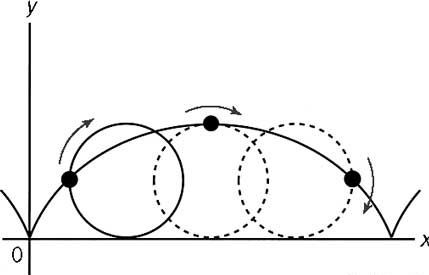
\includegraphics[width=8cm]{images/04_analisis2/cicloide.png}
\end{center}

Dicha curva puede parametrizarse por

\begin{eqnarray*} g : \RR &\to& \RR^2 \\
g(t) &=& a ( t - \sin(t) , 1 - \cos(t) ) \end{eqnarray*}

la cual es derivable en todo su dominio, su derivada es

$$ g'(t) =  a ( 1 - \cos(t), \sin(t) ) $$

Calculemos algunos puntos de la curva

\begin{eqnarray*}X_0 &=& g(0) = (0, 0) \\
X_1 &=& g(\pi/2) = a (\pi/2 - 1, 1) \\
X_2 &=& g(\pi) = a ( \pi, 2) \\
X_3 &=& g(2\pi) = a ( 2\pi, 0) \end{eqnarray*}

Veamos cuales de ellos son regulares

\begin{eqnarray*} g'(0) &=& a ( 0, 0 ) \\
g'(\pi/2) &=& a (1, 1) \\
g'(\pi) &=& a (2, 0) \\
g'(2\pi) &=& a (0, 0) \end{eqnarray*}

Por lo tanto los puntos $ X_1$ y $X_2$ son regulares, y los puntos $ X_0$ y $X_3$ no lo son (se dice que son singulares).  Además en $X_2$ el vector tangente es \emph{horizontal}, de hecho la recta tangente en dicho punto es la recta horizontal de ecuación $y = 2a$
\end{example}


% % % % % % % % % % % % % % % % % % % % % % % % % % % % % %

\chapter{Diferenciabilidad}

En Análisis 1, si una función era derivable en un punto, entonces también era contínua en él.

En Análisis 2, nuestra definición de función derivable en un punto, para funciones de más de una variable, es tal que puede ser derivable en un punto (en toda dirección y sentido), y aún así no ser contínua en él. 

Hay muchos ejemplos donde esto ocurre, veamos uno sencillo:

Dada $f(x,y) = \begin{cases} x^2/y & y \neq 0 \\ 0 & y=0 \end{cases}$, veamos si es derivable en $(0,0)$.  Sea $v = (a,b)$, luego

$$ \lim_{h \to 0} \frac{f((0,0) + h(a,b)) - f(0,0)}{h} $$

$$ \lim_{h \to 0} \frac{f(ha,hb) - f(0,0)}{h} $$

Si $b = 0$

$$ \lim_{h \to 0} \frac{0 - 0}{h} = 0 $$

Si $b \neq 0$

$$ \lim_{h \to 0} \frac{ \left( \frac{h^2 a^2}{hb} \right) - 0 }{h} = \frac{a^2}{b} $$

Luego la función es derivable en $(0,0)$ y sus derivadas valen

$$ f'((0,0),(a,b)) = \begin{cases} \frac{a^2}{b} & b \neq 0 \\ 0 & b = 0 \end{cases}$$

Pero esta función no es contínua en $(0,0)$ pues $f(0,0) = 0$, pero si nos restringimos al camino $y = x^2$ tenemos

$$ \lim_{ x \to 0 \ y=x^2 } f(x,y) = \lim_{x \to 0} \frac{x^2}{x^2} = 1 \neq 0$$

Por lo tanto la función no es contínua en $(0,0)$.

La idea de esta sección es generalizar la idea de derivada de Análisis 1 en un nuevo concepto que vamos a llamar diferenciabilidad, de forma tal que este nuevo concepto implique continuidad, así como lo hacía el concepto de derivabilidad en una variable.

Primero recordemos la definición de función derivable en un punto de Análisis 1.

\begin{definition}
Una función escalar $ f : A \subset \RR \to \RR$ es derivable en $ x_0 \in A^{\circ}$ si existe el siguiente límite

$$ f'(x_0) = \lim_{h \to 0} \frac{f(x_0 + h) - f(x_0)}{h} $$
\end{definition}

Pero esto equivale a pedir

$$ \lim_{h \to 0} \frac{f(x_0 + h) - f(x_0) - h f'(x_0)}{h} = 0 $$

O sea es derivable sii existe una función escalar $ \mu : A \to \RR$ tal que

$$ f(x_0 + h) - f(x_0) - f'(x_0) h = h \mu(h) $$

con 

$$ \lim_{h \to 0} \mu(h) = 0$$

Por otro lado, la expresión $ f'(x_0) h$ es una transformación lineal $T : \RR \to \RR$, $h \to T(h)$.

Por lo tanto podemos decir que $f$ es derivable sii existe una transformación lineal $T : \RR \to \RR$ y un campo escalar $ \mu : A \to \RR$ tales que

$$ f(x_0 + h) - f(x_0) = T(h) + h \mu(h)$$

con 

$$ \lim_{h \to 0} \mu(h) = 0$$

Ahora sí estamos en condiciones de definir función diferenciable en un punto:

\section{Definición de función diferenciable}

\begin{definition}[Diferenciabilidad]
Un campo vectorial $ f : A \subseteq \RR^n \to \RR^m$ se dice que es una \textbf{función diferenciable en $ x_0 \in A^{\circ} $} \index{Diferenciabilidad} si existe una transformación lineal $ T : \RR^n \to \RR^m$ y un campo vectorial $ \mu : B(x_0, \delta) \cap A \to \RR^m$ tales que

$$ f(x_0 + h) - f(x_0) = T(h) + ||h|| \mu(h) $$

con 

$$  \lim_{h \to 0} \mu(h) = 0 $$

A la transformación lineal asociada $T$ la llamamos el \textbf{diferencial de $f$ en $x_0$}.

\end{definition}
Esta definición tiene concecuencias importantes.  Veremos algunas de ellas en las siguientes secciones.

\section{Diferenciabilidad implica Derivabilidad}

\begin{theorem} \label{difderiv}
Sea el campo vectorial $ f : A \subset \RR^n \to \RR^m$ diferenciable en $ x_0 $, entonces $f$ es derivable en $x_0$, y además las derivadas valen 

$$ f'(x_0, \hat{v}) = D f(x_0) \cdot \hat{v}$$
\end{theorem}

\begin{proof}
Como $f$ es diferenciable en $x_0$ existen una transformación lineal $T : \RR^n \to \RR^m$ y un campo vectorial $ \mu : \RR^n \to \RR^m$ tales que

$ \displaystyle f(x_0 + h) - f(x_0) = T(h) + ||h|| \mu(h)$

Considerando $ h = k\hat{v}$

$ \displaystyle f(x_0 + k\hat{v}) - f(x_0) = T(k\hat{v}) + ||k \hat{v}|| \mu(k\hat{v})$

$ \displaystyle f(x_0 + k\hat{v}) - f(x_0) = k T(\hat{v}) + |k| \mu(k\hat{v})$

dividiendo por $k$ y tomando límite $ k \to 0 $

$ \displaystyle \lim_{k \to 0} \frac{f(x_0 + k\hat{v}) - f(x_0)}{k} = \lim_{k \to 0} T(\hat{v}) + \frac{|k|}{k} \mu(k \hat{v})$

Y como $T(\hat{v})$ no depende de $k$, y como $\frac{|k|}{k}$ es acotada y $\mu \to 0$, se tiene

$ \displaystyle f'(x_0, \hat{v}) = T(\hat{v}) $
\end{proof}

\begin{corollary}
Sea un campo vectorial $ f : A \subset \RR^n \to \RR^m$ diferenciable en $x_0 \in A^{\circ}$, y sea $T$ una transformación lineal que cumple lo pedido, entonces dicha transformación lineal es única, y además 

$$ T(\hat{e_i}) = f'(\vec{x_0}, \hat{e_i})$$  
\end{corollary}

\begin{proof}
Por el teorema anterior $ f'(\vec{x_0}, \hat{v}) = T(\hat{v}) $.  Haciendo $ v = e_i$ tenemos $ f'(\vec{x_0}, \hat{e_i}) = T(\hat{e_i}) $.  

Para ver que la transformación lineal es única, como $\{e_i\}_{1 \leq i \leq n}$ es una base de $\RR^n$, cualquier vector $x \in \RR^n$ lo puedo escribir en forma única como combinación lineal $x = \sum_{i=1}^n \lambda_i e_i$, luego si $T : \RR^n \to \RR^m$ es una transformación lineal debe cumplir $T(x) = \sum_{i=1}^n \lambda_i T(e_i)$, y por lo visto recién debe cumplir  $T(x) = \sum_{i=1}^n \lambda_i f'(x_0, e_i)$, con lo cual quedó complétamente determinada, es decir la transformación lineal es única.
\end{proof}

\begin{definition}[Jacobiana]
Sea $f : A \subseteq \RR^n \to \RR^m$  diferenciable en $x_0 \in A^{\circ}$, de la forma $ f = (f_1, f_2, \ldots, f_m)$, y sea $T : \RR^n \to \RR^m$ el diferencial de $f$ en $x_0$.

Sea $[T]$ la matriz asociada a la transformación lineal $T$ respecto a las bases canónicas de $\RR^n$ y $\RR^m$.  La misma se expresa poniendo en sus columnas los transformados de la base canónica, es decir las derivadas parciales de $f$ en $x_0$, es decir que

$$ [T] = \begin{pmatrix} f'_{1, e_1} & f'_{1, e_2} & \ldots & f'_{1, e_n} \\ f'_{2, e_1} & f'_{2, e_2} & \ldots & f'_{2, e_n} \\ \ldots \\ f'_{m, e_1} & f'_{m, e_2} & \ldots & f'_{m, e_n} \end{pmatrix} $$

Al diferencial $T$ de $f$ en $x_0$ lo vamos a denotar también $df$.  Y a la matriz $[T]$ asociada al diferencial la vamos a llamar la \textbf{matriz jacobiana de $f$ en $x_0$}, \index{Diferenciabilidad!Matriz Jacobiana} y la denotamos $Df(x_0)$.
\end{definition}

\section{Diferenciabilidad implica Continuidad}

\begin{theorem}
Sea el campo vectorial $ f : A \subset \RR^n \to \RR^m$ diferenciable en $ x_0 \in A^{\circ}$, entonces $f$ es contínuo en $x_0$.
\end{theorem}

\begin{proof}
Como $ f$ es diferenciable en $x_0$ existen una (única) transformación lineal $ T : \RR^n \to \RR^m$ y un campo vectorial $ \mu : A \to \RR^m$ tales que

$$ f(x_0 + h) - f(x_0) = T(h) + ||h|| \mu(h) $$

Tomando límite $h \to 0$

$$ \lim_{h \to 0} f(x_0 + h) - f(x_0) = \lim_{h \to 0} \underbrace{T(h)}_{\to 0} + \underbrace{||h||}_{\to 0} \underbrace{\mu(\vec{h})}_{\to 0}$$

O sea

$$ \lim_{h \to 0} f(x_0 + h) - f(x_0) = 0 $$

$$ \lim_{h \to 0} f(x_0 + h) = f(x_0) $$

Sustituyendo $ x = x_0 + h$ queda $ h = x - x_0$, y cuando $ h \to 0$ se tiene $x \to x_0$, reemplazando:

$$ \lim_{x \to x_0} f(x) = f(x_0) $$

lo cual nos dice que el límite existe y es igual al valor de la función en el punto, o sea que $f$ es contínua en $x_0$.
\end{proof}

\section{Gradiente}

\begin{definition}[Gradiente]
Sea el campo escalar $ f : A \subset \RR^n \to \RR^m$, y $x_0 \in A^{\circ}$, si existen las derivadas parciales de $f$ en $x_0$, definimos el \textbf{vector gradiente $\nabla f(x_0)$ de $f$ en $x_0$} \index{Diferenciabilidad!Gradiente} como el vector cuyas coordenadas son las derivadas parciales de $f$ en $x_0$, es decir como

$$ \nabla f(x_0) = (f'_{e_1}(x_0), f'_{e_2}(x_0), \ldots, f'_{e_n}(x_0) ) $$

\end{definition}

\begin{observation} \label{graderiv}

Sea el campo escalar $ f : A \subset \RR^n \to \RR^m$, diferenciable en $x_0 \in A^{\circ}$, y sea $v \in \RR^n$. El teorema \ref{difderiv} nos dice en este caso que

$$ f'_v(x_0) = \nabla f(x_0) \cdot v $$

\end{observation}

\section{El gradiente es normal al conjunto de nivel}

\begin{observation}
Sea el campo escalar $ f : A \subset \RR^n \to \RR$ diferenciable en $x_0 \in A^{\circ}$, y sea $ k \in \RR$, entonces $ \nabla f(x_0)$ es perpendicular al conjunto de nivel $k$ de $f$.
\end{observation}

\begin{proof}

El conjunto de nivel $k$ de $f$ son los $x \in A$ tales que

$$ f(x) = k $$

Sea $ g:[a,b] \to \RR^n$ la parametrización de una curva incluída en el conjunto de nivel, es decir que $g([a,b]) \subseteq C_k(f)$, tal que $g(t_0) = x_0$ y $g'(t_0) \neq 0$.

Entonces podemos componer $g$ con $f$ y obtenemos

$$ f(g(t)) = k $$

Aplicando el teorema \ref{regla_cadena} (la regla de la cadena, que vamos a ver después) se tiene

$$ \nabla f(g(t)) \cdot g'(t) = 0 $$

Es decir que $ \nabla f(x_0) \cdot g'(t_0) = 0$, o sea que $ f(x_0) \perp g'(t_0)$.  

Pero $ g'(t_0)$ es un vector director de la recta tangente una curva que está incluída en el conjunto de nivel, es decir es paralelo al conjunto de nivel, y por lo tanto el gradiente es normal al conjunto de nivel.

\end{proof}

\section{Direcciones de derivada máxima, mínima y nula}

\begin{proposition}
Sea $ f : A \subset \RR^n \to \RR$ es diferenciable en $ x_0 $ y $\nabla f(x_0) \neq 0$.  Entonces:

\begin{itemize}
\item Existe una única dirección de máxima derivada direccional y es $r_{max} = \frac{\nabla f(x_0)}{||\nabla f(x_0)||}$.  El valor de dicha derivada es $||\nabla f(x_0)||$.

\item Existe una única dirección de mínima derivada direccional y es $r_{min} = - r_{max}$.  El valor de dicha derivada es $ - ||\nabla f(x_0)||$.

\item Si además $n=2$, entonces existen exactamente dos direcciones de derivada direccional nula, y si $\nabla f(x_0) = (a,b)$ entonces las mismas son $r_1 = \frac{(-b,a)}{||(-b,a)||}$ y $r_2 = - r_1$
\end{itemize}

\end{proposition}

\begin{proof}

Como $f$ es diferenciable en $x_0$, por la observación \ref{graderiv} sabemos que $f$ es derivable en $x_0$ y

$$ f'_v(x_0) = \nabla f(x_0) \cdot v $$

Pero

\[ \nabla f(x_0) \cdot v = \underbrace{|| \nabla f(x_0)||}_{cte} \underbrace{||v||}_{=1} \underbrace{\cos(\phi)}_{\in [-1,1]} \]

donde $\phi$ es el ángulo entre $\nabla f(x_0)$ y $v$.

Para que dicha derivada sea máxima se requiere $ \cos(\phi) = 1$, por lo tanto el valor máximo que toma es $ || \nabla f(x_0)||$, y esto ocurre cuando el ángulo es 0, es decir cuando $v = r_{max} = \frac{\nabla f(x_0)}{||\nabla f(x_0)||}$

Por la propiedad de homogeneidad, la mínima derivada direccional es $ - || \nabla f(x_0)||$ y ocurre en la dirección $v = r_{min} = - r_{max}$

Finalmente, supongamos que $n=2$, y buscamos las direcciones de derivada direccional nula, es decir tales que

$$ f'_v(x_0) = 0 = \nabla f(x_0) \cdot v$$

Es decir estamos buscando los versores normales a $\nabla f(x_0)$.  

Dado el vector $\nabla f(x_0) = (a,b)$, una forma fácil de encontrar un vector normal es intercambiar las coordenadas y cambiarle el signo a una.  Luego dividimos por la norma y obtuvimos un versor normal.  El otro es símplemente el opuesto aditivo.  Es decir las direcciones de derivada direccional nula son

$$ v_{nul_1} = \frac{(-b,a)}{||(a,b)||} $$

y 

$$ v_{nul_2} = - v_{nul_1} $$
\end{proof}

\section{$C^1$ implica diferenciable}

\begin{theorem}
Sea el campo escalar $ f : A \subset \RR^n \to \RR^m$ con $A$ abierto.
Si $ f \in C^1$, entonces $f$ es diferenciable en todo $x \in A$.
\end{theorem}

\begin{observation}
Una función $f$ puede ser diferenciable y aún así $ f \not\in C^1$.
\end{observation}

Por ejemplo, la siguiente función es diferenciable en $\RR$, pero su derivada $f'(x)$ no es contínua en el origen.

$$ f(x) = \begin{cases} x^2 \sin(\frac{1}{x}) & si \ x \neq 0 \\ 0 & si \ x=0 \end{cases} $$

% % % % % % % % % % % % % % % % % % % % % % % % % % % % % %

\chapter{Funciones Compuestas e Implícitas}

\section{Función Compuesta}

\begin{definition}
Sean $ f : A \subset \RR^n \to \RR^m$ y $ g : B \subset \RR^m \to \RR^p$ tales que $f(A) \subseteq B$.

Entonces existe una única la función $ h : A \to \RR^p$ tal que $h(x) = g(f(x))$.  

A dicha función $h$ la llamamos la \textbf{función compuesta de $f$ con $g$}, y la denotamos como 

$$ h = g \circ f$$
\end{definition}

Notar que esta definición es un poco más general que la definición \ref{funcion_compuesta}, por cuanto no se pide que el codominio de la primera sea igual al dominio de la segunda, sólo que la imagen de la primera esté incluído en el dominio de la segunda.

Al mismo tiempo es más particular que aquella definición, pues la primera se refiere funciones entre conjuntos en general, mientras que la segunda es entre subconjuntos de $\RR^n$.

\section{Regla de la Cadena}

\begin{theorem}[Regla de la cadena] \label{regla_cadena} \index{Diferenciabilidad!Regla de la cadena}
Sean $ f : A \subset \RR^n \to \RR^m$ diferenciable en $x_0 \in A^{\circ}$, y $ g : B \subset \RR^m \to \RR^p$ diferenciable en $y_0 = f(x_0) \in B^{\circ}$, tales que $f(A) \subseteq B$

Entonces la función compuesta $h : A \to \RR^p$ es diferenciable en $x_0$, y además el diferencial de $h$ en $x_0$ es igual a la composición de los diferenciales de $f$ en $x_0$ con el de $g$ en $y_0$, de la siguiente manera

$$ dh(x_0) = dg(y_0) \circ df(x_0) $$

O lo mismo expresado matricialmente, la matriz jacobiana de la compuesta es igual al producto de las matrices jacobianas de la siguiente manera

$$ Dh(x_0) = Dg(y_0) \cdot Df(x_0) $$
\end{theorem}

\section{Función definida implícitamente}

\begin{definition}
Dada una función $F : A \subseteq \RR^{n+1} \to \RR$, decimos que la ecuación $F(x_1, x_2, \ldots, x_n, y) = 0$ \textbf{define implícitamente a $y$ como función de $x_1, \ldots, x_n$ en $B$} si existe una función $ f : B \subseteq \RR^n \to \RR$ tal que $F(x_1, \ldots, x_n, f(x_1, \ldots, x_n)) = 0$, para $B \subseteq A_y$ donde $A_y$ es la proyección de $A$ sobre $x_1, \ldots, x_n$
\end{definition}

Ejemplo: $F: \RR^3 \to \RR$, $F(x,y,z) = x^2 + y^2 - z$.  La ecuación correspondiente es $x^2 + y^2 - z = 0$. Como existe $f : \RR^2 \to \RR$, $f(x,y) = x^2 + y^2$ tal que $F(x,y,f(x,y)) = 0$, la ecuación define implícitamente a $z$ como función de $x,y$.

Otro ejemplo: $F: \RR^3 \to \RR$, $F(x,y,z) = x^2 + y^2 + z^2 - 1$.  La ecuación correspondiente es $x^2 + y^2 + z^2 = 1$. 

Sea $D_2 = \{ (x,y) \in \RR^2 : x^2 + y^2 \leq 1 \}$. Como existe $f : D_2 \subseteq \RR^2 \to \RR$, $f(x,y) = \sqrt{1 - x^2 + y^2}$ tal que $F(x,y,f(x,y)) = 0$, la ecuación define implícitamente a $z$ como función de $x,y$.

Notar que globálmente la relación entre $x,y$ y $z$ no es funcional, pues por ejemplo tanto el $(0,0,1)$ como el $(0,0,-1)$ satisfacen la ecuación, pero $f(0,0)$ debe tener una única imagen.  En particular, la función definida implícitamente no tiene porqué ser única, otra función definida implícitamente por la misma ecuación es $g : D_2 \to \RR^2$, $g(x,y) = - \sqrt{1 - x^2 - y^2}$

\section{Teorema de Cauchy-Dini}

\begin{theorem}{Teorema de Cauchy-Dini} \label{cauchy_dini} \index{Diferenciabilidad!Teo. Cauchy-Dini}
Sea $F : A \subseteq \RR^{n+1} \to \RR$ con $A$ abierto y $F \in C^1$, y sea la ecuación $F(x_1, \ldots, x_n, y) = 0$.

Sea además $P=(a_1, \ldots, a_n, y_0) \in A$, tal que $F(P) = 0$, y $ F'_y(P) \neq 0$.  

Entones la ecuación define implícitamente a $y$ como función de $x_1, \ldots, x_n$ en un entorno de $P_y = (a_1, \ldots, a_n)$, y resulta que $ f $ es diferenciable en $P_y$, y además

$$ f'_{x_i}(P_y) = - \frac{F'_{x_i}(P)}{F'_y(P)} $$
\end{theorem}

Este teorema nos garantiza bajo ciertas condiciones la existencia de una función definida implícitamente, es decir que exista $ f : A_y \cap E(P_y, \delta) \subset \RR^n \to \RR$ tal que $F(x_1, \ldots, x_n, f(x_1, \ldots, x_n)) = 0$

En particular, esto nos permite el gradiente $ \nabla f(P_y)$ de la siguiente manera

$$ \nabla f(P_y) = \left( - \frac{F'_{x_1}(P)}{F'_y(P)}, - \frac{F'_{x_2}(P)}{F'_y(P)}, \ldots, - \frac{F'_{x_n}(P)}{F'_y(P)} \right) $$

$$ = - \frac{1}{F'_y(P)} \left( F'_{x_1}(P), F'_{x_2}(P), \ldots, F'_{x_n}(P) \right) $$

% % % % % % % % % % % % % % % % % % % % % % % % % % % % % %

\chapter{Polinomio de Taylor y Extremos}

\section{Polinomio de Taylor}

Sea $f: A \subseteq \RR^2 \to \RR$, $f \in C^2$, $(x_0, y_0) \in A$.

Sabemos que el diferencial de $f$ en cada punto $(x_0, y_0) \in A$ es de la forma

$$ df_{(x_0,y_0)}(x-x_0, y-y_0) = f'_x(x_0,y_0) (x-x_0) + f'_y(x_0,y_0) (y-y_0) $$

O escribiendo $(u,v) = (x-x_0, y-y_0)$

$$ df_{(x_0,y_0)}(u,v) = f'_x(x_0,y_0)u + f'_y(x_0,y_0)v $$

En cada punto $(x,y)$ su diferencial es

$$ df_{(x,y)}(u,v) = f'_x(x,y)u + f'_y(x,y)v $$

Ahora definimos el diferencial segundo de $f$ en $(x,y)$, como el diferencial del diferencial, es decir

\begin{eqnarray*} d^2 f_{(x,y)}(u,v) = d( df_{(x,y)}(u,v) ) &=& d( f'_x(x,y)u + f'_y(x,y)v ) \\ 
&=& f''_{xx}(x,y)u^2 + f''_{xy}(x,y)uv + f''_{yx}(x,y)vu + f''_{yy}(x,y)v^2 \\
&=& f''_{xx}(x,y)u^2 + 2 f''_{xy}(x,y)uv + f''_{yy}(x,y)v^2 \end{eqnarray*}

donde en el último paso usamos el teorema \ref{schwarz} (de Schwarz).

Con esta notación vamos a definir entonces el polinomio de Taylor

\begin{definition}[Taylor] \index{Diferenciabilidad!Polinomio de Taylor} 
Sea $f: A \subseteq \RR^2 \to \RR$, $f \in C^2$, $(x_0, y_0) \in A$.

El \textbf{polinomio de Taylor de primer grado de $f$ en $(x_0, y_0)$} es

\begin{eqnarray*} T_1(x,y) &=& f(x_0,y_0) + df_{(x_0, y_0)}(x-x_0,y-y_0) \\ 
&=& f(x_0,y_0) + f'_x(x_0,y_0)(x-x_0) + f'_y(x_0,y_0)(y-y_0) \end{eqnarray*}

Y el \textbf{polinomio de Taylor de segundo grado de $f$ en $(x_0, y_0)$} es

\begin{eqnarray*} T_2(x,y) &=& f(x_0,y_0) + df_{(x_0,y_0)}(x-x_0,y-y_0) + \frac{1}{2!} d^2f_{(x_0,y_0)}(x-x_0,y-y_0) \\ 
&=& f(x_0,y_0) + f'_x(x_0,y_0)(x-x_0) + f'_y(x_0,y_0)(y-y_0) + \\
&+& \frac{1}{2!} \left[ f''_{xx}(x_0,y_0)(x-x_0)^2 + 2 f''_{xy}(x_0,y_0)(x-x_0)(y-y_0) + f''_{yy}(x_0,y_0)(y-y_0)^2 \right] \end{eqnarray*}

Más generalmente, si $f : A \subseteq \RR^n \to \RR$, $f \in C^k$, $x_0 \in A$, y llamando $u = x - x_0$, el \textbf{polinomio de Taylor de $f$ de grado $k$ en $x_0$} es

$$ T_k(x) = f(x_0) + df_{x_0}(x-x_0) + \frac{1}{2!} d^2f_{x_0}(x-x_0) + \ldots + \frac{1}{k!}d^kf_{x_0}(x-x_0) $$
\end{definition}

El polinomio de Taylor sirve para aproximar la función en un entorno del punto donde fué calculada.  Es decir si $f \in C^k$ y $T_k(x)$ es el polinomio de grado $k$ de $f$ en $x_0$, entonces

$$ f(x) \approx T_k(x)$$

para $x$ \emph{cerca} de $x_0$.

Más precisamente, se verifica que

$$ \lim_{x \to x_0} \frac{ f(x) - T_k(x) }{ ||x-x_0||^k } = 0$$

\section{Máximos y mínimos de una función}

Sabemos que $\RR$ es un conjunto totalmente ordenado (ver definición \ref{orden_total}), y por lo tanto cualquier subconjunto $B \subseteq \RR$ también hereda un orden total.

Tiene sentido entonces para $B \subseteq \RR$ preguntar si tiene un máximo o un mínimo.

Por ejemplo, si $A = (0,1]$, entonces $A$ tiene un máximo y es el elemento $1 \in A$, pero no tiene ningún mínimo.

\begin{definition}[Máximo absoluto] \index{Extremos!Absolutos}
Sea $f : A \subseteq \RR^n \to \RR$ un campo escalar, y sea $Y = Im(f) \subseteq \RR$ el conjunto imagen de $f$.  

Si $Y$ tiene un máximo, decimos que es el \textbf{máximo absoluto de $f$}.  

Si $Y$ tiene un mínimo, decimos que es el \textbf{mínimo absoluto de $f$}.  
\end{definition}

\begin{definition}[Máximo relativo] \index{Extremos!Relativos}
Sea $f : A \subseteq \RR^n \to \RR$ un campo escalar, $x_0 \in A$, $E = E(x_0, \delta)$ un entorno de $x_0$ de radio $\delta > 0$, y $g = f|_{E}$, es decir la función $f$ restringida al entorno $E$, y sea $Y_E = Im(g)$ la imagen de la función así restringida.

Si $Y_E$ tiene un máximo, decimos que es un \textbf{máximo relativo de $f$ relativo a $x_0$}.

Si $Y_E$ tiene un mínimo, decimos que es un \textbf{mínimo relativo de $f$ relativo a $x_0$}.
\end{definition}

\begin{definition}[Extremos]
Llamamos \textbf{extremos} a los máximos y mínimos (absolutos y relativos) de $f$.
\end{definition}

\begin{observation}
Las definiciones anteriores las podemos expresar también de la siguiente manera.

Sea el campo escalar $ f : A \subset \RR^n \to \RR$, y $ x_0 \in A$, entonces:

$ f(x_0)$ es el \textbf{máximo absoluto de $f$} si $ f(x) \leq f(x_0)$ para todo $x \in A$

$ f(x_0)$ es el \textbf{mínimo absoluto de $f$} si $ f(x) \geq f(x_0)$ para todo $x \in A$

$ f(x_0)$ es \textbf{máximo relativo de $f$ relativo a $x_0$} si $ f(x) \leq f(x_0)$ para todo $x \in A \cap E(x_0, \delta)$ para algún $\delta > 0$

$ f(x_0)$ es \textbf{mínimo relativo de $f$ relativo a $x_0$} si $ f(x) \geq f(x_0)$ para todo $x \in A \cap E(x_0, \delta)$ para algún $\delta > 0$
\end{observation}

\begin{observation}
Todos los extremos se definieron en \textbf{sentido amplio}. La definición en \textbf{sentido estricto} es análoga pero cambiando $\leq$ por $<$ y $\geq$ por $>$, y analizando $A - \{x_0\}$ para extremos absolutos, y $( A - \{x_0\} ) \cap E(x_0, \delta)$ para extremos relativos.
\end{observation}

\subsection{Criterio de la derivada primera}

Antes de enunciar el criterio, vamos a necesitar esta

\begin{definition}[Punto crítico/silla] \label{punto_critico_silla}
Sea $f : A \subset \RR^n \to \RR$.  Un \textbf{punto crítico de $f$} \index{Extremos!Punto crítico} es un elemento $x_0 \in A$ tal que o bien $f$ no es diferenciable en $x_0$, o bien es diferenciable en $x_0$ pero $ \nabla f(x_0) = 0$.

Si $x_0$ es punto crítico, pero $f(x_0)$ no es extremo, decimos que $(x_0, f(x_0))$ es \textbf{punto silla}. \index{Extremos!Punto silla}
\end{definition}

Ahora si enunciamos el criterio de la derivada primera

\begin{theorem}[Criterio de la derivada primera] \label{criterio_derivada_primera} \index{Extremos!Criterio derivada primera}
Sea $f : A \subset \RR^n \to \RR$, tal que $f(x_0)$ es extremo.  Entonces $x_0$ es punto crítico.

Es decir que una condición necesaria para que $f(x_0)$ sea extremo, es que $x_0$ sea punto crítico.
\end{theorem}

En otras palabras si $x_0 \in A$ es punto crítico, entonces o bien $f(x_0)$ es extremo, o bien $(x_0, f(x_0))$ es punto silla.

\begin{proof}
Sea $g(t) = x_0 + t v$ para un versor $v \in \RR^n$, y considero la composición 

$$h(t) = f(g(t))$$  

Como $g(0) = x_0$ y $f$ presenta un extremo en $x_0$, entonces $h$ presenta un extremo en $0$. 

Además como $f$ es diferenciable en $x_0$ y $g$ es diferenciable en $0$, entonces por la regla de la cadena $h$ es diferenciable en $0$ y

$$ h'(0) = \nabla f(g(0)) g'(0) $$

Y por el criterio de la derivada primera (de Análisis 1) sabemos que debe cumplirse 

$$ h'(0) = 0$$

O sea que

$$ \nabla f(g(0)) \cdot g'(0) = 0 $$

Pero $g'(0) = v$, luego nos queda

$$ \nabla f(x_0) \cdot v = 0$$

y como $f$ es diferenciable en $x_0$ 

$$ \nabla f(x_0) \cdot v = f'_v(x_0) = 0 $$

En particular tomando $v$ un versor \emph{canónico} de $\RR^n$ vemos que todas las derivadas parciales son nulas, y por lo tanto $ \nabla f(x_0) = 0$ como queríamos probar.
\end{proof}

\subsection{Criterio de la derivada segunda}

Antes de enunciar el criterio de la derivada segunda nos va a ser útil la siguiente

\begin{definition}[Matriz Hessiana]
Sea $f : A \subset \RR^n \to \RR$, $f \in C^2$.

La \textbf{matriz Hessiana} \index{Extremos!Matriz Hessiana} es la matriz jacobiana del gradiente de $f$.  Es decir:

$$ Hf = \begin{pmatrix} f''_{x_1 x_1} & f''_{x_1 x_2} & \ldots & f''_{x_1 x_n} \\ f''_{x_2 x_1} & f''_{x_2 x_2} & \ldots & f''_{x_2 x_n} \\ \ldots \\ f''_{x_n x_1} & f''_{x_n x_2} & \ldots & f''_{x_n x_n} \end{pmatrix} $$

\end{definition}

\begin{observation} \label{hessiana_simetrica}
Por el teorema \ref{schwarz} (de Schwarz), la matriz Hessiana debe ser simétrica.
\end{observation}

\begin{theorem} \label{hermite}
Sea $M \in \RR^{n \times n}$ una matriz cuadrada y simétrica.

Entonces $M$ tiene autovalores $\lambda_1, \lambda_2, \ldots, \lambda_n \in \RR$, es decir tiene todos sus autovalores y son reales.
\end{theorem}

\begin{definition} \label{definida_positiva}

Sea $M \in \RR^{n \times n}$ una matriz cuadrada y simétrica con coeficientes reales.

Sabemos por el teorema \ref{hermite} que todos sus autovalores $\lambda_1, \ldots, \lambda_n$ son reales.

Decimos que $M$ es una \textbf{matriz definida positiva}, si todos sus autovalores son positivos, es decir $\lambda_i > 0$ para $1 \leq i \leq n$.

Decimos que $M$ es una \textbf{matriz semidefinida positiva}, si todos sus autovalores son no negativos, es decir $\lambda_i \geq 0$ para $1 \leq i \leq n$.

Decimos que $M$ es una \textbf{matriz definida negativa}, si todos sus autovalores son negativos, es decir $\lambda_i < 0$ para $1 \leq i \leq n$.

Decimos que $M$ es una \textbf{matriz semidefinida negativa}, si todos sus autovalores son no positivos, es decir $\lambda_i \leq 0$ para $1 \leq i \leq n$.

Decimos que $M$ es una \textbf{matriz no definida}, si no es definida positiva, ni semidefinida positiva, ni definida negativa, ni semidefinida negativa.  Es decir si tiene autovalores tanto positivos como negativos.
\end{definition}

\begin{theorem}[Criterio de Sylvester] \label{sylvester}

Sea $M \in \RR^{n \times n}$ una matriz cuadrada y simétrica.

Sean las $n$ submatrices $M_p = (a_{ij})_{1 \leq i,j \leq p}$ con $1 \leq p \leq n $.

A sus determinantes $det(M_p)$ con $1 \leq p \leq n$ se los conoce somo sus \textbf{menores principales}.

El criterio de Sylvester dice que 

\begin{itemize}
\item $M$ es \emph{definida positiva} sii todos sus menores principales son positivos, es decir $det(M_p) > 0$ para $1 \leq p \leq n$

\item $M$ es \emph{definida negativa} sii sus menores principales son de la forma $det(M_1)<0, det(M_2)>0, det(M_3)<0, \ldots$, es decir $(-1)^p det(M_p) > 0$ para $1 \leq p \leq n$.  Es decir van intercambiando signo empezando por negativo.
\end{itemize}
\end{theorem}

No lo encontré en la bibliografía, y no estoy seguro de si será cierto, pero se me ocurre que a lo mejor también es cierto lo siguiente:

\begin{itemize}
\item $M$ es \emph{semidefinida positiva} sii todos sus menores principales son no negativos, es decir $det(M_p) \geq 0$ para $1 \leq p \leq n$

\item $M$ es \emph{semidefinida negativa} sii sus menores principales son de la forma $det(M_1) \leq 0, det(M_2) \geq 0, det(M_3) \leq 0, \ldots$, es decir $(-1)^p det(M_p) \geq 0$ para $1 \leq p \leq n$.

\item $M$ es no definida sii tiene menores principales tanto positivos como negativos.
\end{itemize}

Ahora si enunciamos el criterio de la derivada segunda

\begin{theorem}[Criterio de la derivada segunda] \label{criterio_derivada_segunda} \index{Extremos!Criterio derivada segunda}

Sea $f : A \subset \RR^n \to \RR$, $ f \in C^2$ y $x_0 \in A$ punto crítico.  Entonces si la matriz hessiana de $f$ en $x_0$ es \emph{definida positiva} (Ver \ref{definida_positiva}), la función presenta un mínimo relativo $f(x_0)$, y si es \emph{definida negativa}, la función presenta un máximo relativo $f(x_0)$.

Si la matriz está semidefinida (positiva o negativa), el criterio no decide.

Si la matriz no está definida, no hay extremo, es decir que $(x_0, f(x_0))$ es punto silla.
\end{theorem}

Combinando el criterio \ref{sylvester} de Sylvester con el criterio \ref{criterio_derivada_segunda} de la derivada segunda, podemos construir el criterio del Hessiano

\begin{theorem}[Criterio del Hessiano] \label{criterio_hessiano}
Sea $f : A \subset \RR^n \to \RR$, $ f \in C^2$ y $x_0 \in A$ punto crítico.

Sean las $n$ submatrices $M_p = (a_{ij})_{1 \leq i,j \leq p}$ con $1 \leq p \leq n $, y sean $det(M_p)$ sus menores principales.

Entonces 

\begin{itemize}
\item Si $det(M_p) > 0$ para $1 \leq p \leq n$, $f(x_0)$ es mínimo relativo.

\item Si $(-1)^p det(M_p) > 0$ para $1 \leq p \leq n$, $f(x_0)$ es máximo relativo.

\item Si algún $det(M_p) = 0$, el criterio no decide.

\item En cualquier otro caso, el punto $(x_0, f(x_0))$ es un punto silla.
\end{itemize}
\end{theorem}

\begin{example}
Veamos el caso particular $n=3$.  Sea $f : A \subseteq \RR^3 \to \RR$, $f \in C^2$ y $x_0 \in A$ punto crítico de $f$.  Queremos saber si $f(x_0)$ es extremo relativo. Sea $Hf(x_0)$ la matriz hessiana de $f$ en $x_0$

$$ Hf(x_0) = \begin{pmatrix} f''_{xx}(x_0) & f''_{xy}(x_0) & f''_{xz}(x_0) \\ f''_{yx}(x_0) & f''_{yy}(x_0) & f''_{yz}(x_0) \\ f''_{zx}(x_0) & f''_{zy}(x_0) & f''_{zz}(x_0) \end{pmatrix} $$

Calculamos los \emph{menores principales} de $f$, es decir los siguientes determinantes (se entiende, todas las funciones evaluadas en $x_0$) 

$$ H_1 = \left| \begin{matrix} f''_{xx} \end{matrix} \right| $$

$$ H_2 = \left| \begin{matrix} f''_{xx} & f''_{xy} \\ f''_{yx} & f''_{yy} \end{matrix} \right| $$

$$ H_3 = \left| \begin{matrix} f''_{xx} & f''_{xy} & f''_{xz} \\ f''_{yx} & f''_{yy} & f''_{yz} \\ f''_{zx} & f''_{zy} & f''_{zz} \end{matrix} \right| $$

Entonces si $H_1, H_2, H_3 > 0$ la matriz está definida positiva, y por lo tanto $f(x_0)$ es mínimo relativo.

Y si $H_1 < 0$, $ H_2 > 0$, $H_3 < 0$ la matriz está definida negativa, y por lo tanto $f(x_0)$ es máximo relativo.

Si algún $H_i = 0$, el criterio no decide.  En cualquier otro caso el punto $(x_0, f(x_0))$ es punto silla.
\end{example}

\begin{example}
Ahora veamos el caso particular $n=2$.  Sea $f : A \subseteq \RR^2 \to \RR$, $f \in C^2$ y $x_0 \in A$ punto crítico de $f$.  Queremos saber si $f(x_0)$ es extremo relativo. Sea $Hf(x_0)$ la matriz hessiana de $f$ en $x_0$

$$ Hf(x_0) = \begin{pmatrix} f''_{xx}(x_0) & f''_{xy}(x_0) \\ f''_{yx}(x_0) & f''_{yy}(x_0)  \end{pmatrix} $$

Los menores principales de $f$ son $ H_1 = f''_{xx}(x_0) $ y $ H_2 = det(Hf(x_0)) $.

\begin{itemize}
\item Si $det(Hf(x_0)) > 0$ hay extremo, pues el producto de los dos autovalores es positivo, es decir que son ambos positivos o ambos negativos.  

En este caso si $f''_{xx}(x_0) > 0$, $f(x_0)$ es mínimo relativo, y si $f''_{xx}(x_0) < 0$, $f(x_0)$ es máximo relativo.  

El caso $f''_{xx}(x_0) = 0$ no puede darse, pues si $det(H(fx_0)) = f''_{xx}f''_{yy} - (f''_{xy})^2 > 0$, entonces $f''_{xx}f''_{yy} > (f''{xy})^2 > 0$, lo cual implica que $f''_{xx} \neq 0$

\item Si $det(Hf(x_0)) < 0$ entonces $(x_0, f(x_0))$ es punto silla, pues el producto de los dos autovalores es negativo, es decir que son de signo contrario.

\item Si $det(Hf(x_0)) = 0$ entonces el criterio no decide, habrá que averiguar de otra forma si se produce extremo o punto silla.
\end{itemize}

\end{example}

\section{Extremos condicionados}

Supongamos que queremos maximizar un campo escalar $f(x,y)$, sujeto a una restricción $g(x,y) = 0$.

Un método consiste, cuando es posible, en despejar $x$ o $y$ (o alguna expresión) de la ecuación $g(x,y) = 0$ de forma tal de reemplazarla en la función $ f(x,y)$ para que quede en función de una variable.

Otra posibilidad sería parametrizar la curva $ g(x,y) = 0$, digamos mediante la función vectorial $ r(t)$, luego componer $h = f \circ r$ y maximizar dicha compuesta $h(t) = f(r(t))$ que es una función de una variable.

Pero si ninguno de los métodos anteriores funciona, debemos recurrir a los \textbf{multiplicadores de Lagrange}: \index{Extremos!Multiplicadores de Lagrange}

Definimos la función de Lagrange:

$$ L(\lambda, x,y) = \lambda g(x,y) + f(x,y)$$

Los puntos críticos (restringidos) los hallamos calculando su gradiente e igualando a cero:

$$ \nabla L(\lambda, x,y) = (0,0,0)$$

de donde

\begin{eqnarray*} g(x,y) &=& 0 \\
\lambda g'_x + f'_x &=& 0 \\
\lambda g'_y + f'_y &=& 0 \end{eqnarray*}

Para cada punto crítico restringido podemos analizar si es extremo analizando geométricamente la función, o usando el hessiano restringido:

$$ H = \begin{pmatrix} 0 & g'_x & g'_y \\ g'_x & f''_{xx} & f''_{xy} \\ g'_y & f''_{yx} & f''_{yy} \end{pmatrix}$$

El criterio del hessiano restringido en este caso dice que 

\begin{itemize}

\item Si $ H_3 < 0$ hay mínimo relativo

\item Si $ H_3 > 0$ hay máximo relativo.

\end{itemize}

 En general, si hay $m$ restricciones, se consideran los menores principales de tamaño $ i \geq 2m+1$.
 
Si $m$ es par y $H_i > 0$ para todo $i$ hay mínimo relativo. Y si $ H_{i} < 0, H_{i+1} > 0, H_{i+2} < 0, \ldots$ hay máximo relativo.

Si $m$ es impar y $H_i < 0$ para todo $i$ hay mínimo relativo.  Y si $ H_i > 0, H_{i+1} < 0, H_{i+2} > 0, \ldots$ hay máximo relativo.


\begin{example}
Analizar los extremos de $f(x,y) = x^2 + y^2$ sujeto a $x=0$.

Primero definimos la función de Lagrange

$$ L(\lambda, x,y) = \lambda x + x^2 + y^2$$

Ahora buscamos los puntos críticos

$$ \nabla L(\lambda, x,y) = (x, \lambda+2x, 2y) = (0,0,0)$$

de donde

\begin{eqnarray*} x &=& 0 \\
\lambda + 2x &=& 0 \\
2y &=& 0 \end{eqnarray*}

El único punto crítico es $ (\lambda, x,y) = (0,0,0)$.  Ahora veamos el hessiano

$$ H = \begin{pmatrix} 0 & 1 & 0 \\ 1 & 2 & 0 \\ 0 & 0 & 2 \end{pmatrix} $$

Como $ H_3 = -2 < 0$ hay mínimo relativo $ f(0,0) = 0$
\end{example}


% % % % % % % % % % % % % % % % % % % % % % % % % % % % % %

\chapter{Integral de Línea y Función Potencial}

\section{Integral de Riemann}

Recordemos la definición de la integral de Riemann

\begin{definition}[Integrable]
Sea $[a,b] \in \RR$ un intervalo compacto, y sea $ P = \{a = x_0 < x_1 < \ldots < x_n = b\}$ una partición de $ [a,b]$.  Sea $f$ una función acotada en $ [a,b]$.  

Notamos 

$$ m_i = \inf_{x \in [x_{i-1},x_i]} f(x) $$

$$ M_i = \sup_{x \in [x_{i-1},x_i]} f(x) $$

$$ \triangle x_i = x_i - x_{i-1}$$

Las sumas superior e inferior de Riemann son

$$ S_p(f) = \sum_{i=1}^n M_i \triangle x_i $$

$$ s_p(f) = \sum_{i=1}^n m_i \triangle x_i $$

Luego definimos

$$ \overline{\int_a^b} f dx = \inf_{p \ part} S_p(f)$$

$$ \underline{\int_a^b} f dx = \sup_{p \ part} s_p(f)$$

donde el ínfimo y el supremo se calcula sobre todas las particiones posibles.

Si son iguales, se nota $ \int_a^b f dx$ y se dice que $f$ es Riemann-integrable en $[a,b]$, y lo denotamos $f \in R$
\end{definition}

\section{Curva regular a trozos, curva de jordan}

\begin{definition}[Jordan]
Una curva $C \in \RR^n$ decimos que es \textbf{regular a trozos} si puede escribirse como $\displaystyle C = \cup_{i=1}^k C_i$ donde cada $C_i$ es una curva regular, y el extremo final de una coincide con el inicial de la siguiente.

Es decir si cada curva $C_i$ está parametrizada por $g_i : [a_i, b_i] \to \RR^n$, entonces $g_i(b_i) = g_{i+1}(a_{i+1})$

Una curva $C$ es \textbf{simple} \index{Curva!Simple} si admite una parametrización inyectiva.

Una curva $C$ es \textbf{cerrada} \index{Curva!Cerrada} si admite una parametrización $g:[a,b] \to \RR^n$ tal que $g(a) = g(b)$

Una curva $C$ se dice cerrada simple, o \textbf{curva de Jordan}, \index{Curva!de Jordan} si admite una parametrización $ g:[a,b] \to \RR^n$ tal que es inyectiva en $ [a,b)$ y $ g(a) = g(b)$
\end{definition}

\section{Integral de línea}

\begin{definition}[Integral de línea] \index{Integral de línea}
Dada una curva $C \in \RR^n$ con parametrización $ g:[a,b] \to \RR^n$, y dado un campo escalar $f : A \subseteq \RR^n \to \RR$ contínuo, tal que $C \in A^{\circ}$, definimos el diferencial de curva escalar como

$$ dc = || g'(t) || dt $$

y definimos la integral de $f$ sobre $C$ como

$$ \int_C f dc = \int_a^b f(g(t)) || g'(t) || dt $$

Definimos la longitud de $C$ como la integral de la función constante 1, es decir

$$ Long(C) = \int_C dc = \int_a^b || g'(t) || dt $$

Dada la misma curva $C$ con misma parametrización $g$, y dado el campo vectorial $f : A \subseteq \RR^n \to \RR^n$ contínuo, tal que $C \in A^{\circ}$, definimos el diferencial de curva vectorial como

$$ dc = g'(t) dt $$

y definimos la integral de $f$ sobre $C$ en este caso también llamado \textbf{circulación} como

$$ \int_C f \cdot dc = \int_a^b f(g(t)) \cdot g'(t) dt$$

En ambos casos decimos que se trata de la integral sobre la curva $C$ desde $g(a)$ hasta $g(b)$
\end{definition}

\section{Campos conservativos}

Dado un campo vectorial $ f: A \subseteq \RR^n \to \RR^n$, con $A$ abierto y $f \in C^1$, podemos preguntarnos si en realidad se trata del gradiente de un campo escalar $\phi : A \subseteq \RR^n \to \RR$, $\phi \in C^2$, tal que $ \nabla \phi = f$.  Esto motiva la siguiente

\begin{definition}[Conservativo] \index{Integral de línea!Campo conservativo}
Dado $ f: A \subseteq \RR^n \to \RR^n$, con $A$ abierto y $f \in C^1$.  

Si existe $\phi : A \subseteq \RR^n \to \RR$, $\phi \in C^2$, tal que 

$$ \nabla \phi = f$$

decimos que $f$ es un \textbf{campo conservativo}, y que $\phi$ es su \textbf{función potencial}. \index{Integral de línea!Campo conservativo!Función potencial}
\end{definition}

\begin{example}{No todos los campos vectoriales son conservativos}

Por ejemplo $f(x,y) = (-y, x)$ no es conservativo.  Si lo fuera, como $f \in C^1$ se tendría una $ \phi \in C^2$ tal que $ \nabla \phi = f$, pero en ese caso sería $\phi'_x = -y$ y $\phi'_y = x$.  Se cumplen las hipótesis del teorema de Schwarz, por lo tanto $ \phi''_{xy} = \phi''_{yx}$ con lo cual llegamos a $ -1 = 1$ lo cual es absurdo, y por lo tanto $f$ no es un campo conservativo.
\end{example}

Es fácil construir ejemplos de campos conservativos, símplemente elegimos un campo escalar $ \phi \in C^2$, y su gradiente es un campo conservativo.  Por ejemplo si $\phi(x,y) = x^2 + y^2$ entonces se tiene que $\nabla \phi(x,y) = f(x,y) = (2x, 2y)$ es un campo conservativo, cuya función potencial es $\phi$.

\section{Teorema de la independencia del camino}

\begin{theorem}[Independencia camino] \index{Integral de línea!Campo conservativo!Teo. ind. camino}
Sea el campo vectorial conservativo $f : A \subset \RR^n \to \RR^n$, y sea $ \phi : A \subset \RR^n \to \RR$ su función potencial. 

Sea $ C \subset A^{\circ}$ una curva regular con parametrización $ g:[a,b] \to \RR^n$.

Entonces 

$$ \int_C f \cdot dc = \phi(g(b)) - \phi(g(a)) $$
\end{theorem}

\begin{proof}
Queremos calcular 

$$\int_C f \cdot dc = \int_a^b f(g(t)) \cdot g'(t) dt$$

Como $ f = \nabla \phi$ se tiene

$$\int_C f \cdot dc = \int_a^b \nabla \phi(g(t)) \cdot g'(t) dt$$

Ahora consideramos la función compuesta $ h = \phi \circ g$, $h(t) = \phi(g(t))$.  La misma existe puesto que la curva está en el dominio de $\phi$.

Como $g \in C^1$ por ser la parametrización de una curva regular, y $\phi \in C^2$ por ser función potencial de $f$, ambas son diferenciables, y podemos aplicar el teorema de la regla de la cadena

$$ h'(t) = \nabla \phi(g(t)) \cdot g'(t) $$

reemplazando en la integral

$$ \int_C f \cdot dc = \int_a^b h'(t) dt $$

y por el teorema fundamental del cálculo de Análisis 1

$$ \int_a^b h'(t) dt = h(b) - h(a) $$

Pero $h = \phi(g(t))$, finalmente

$$\int_C f \cdot dc = \phi(g(b)) - \phi(g(a))$$

Es decir que la integral de $f$ sobre la curva $C$ no depende del camino, sino sólamente de los puntos inicial $g(a)$ y final $g(b)$ de la curva. $\qedhere$
\end{proof}

\begin{corollary}
Si $f$ es conservativo, la integral sobre cualquier curva cerrada da cero.
\end{corollary}

\begin{proof}
Como $C$ es cerrada $ g(a) = g(b)$, y como $f$ es conservativo se tiene

$$ \int_C f \cdot dc = \phi(g(b)) - \phi(g(a)) = \phi(g(a)) - \phi(g(a)) = 0$$ 
\end{proof}

\section{Condición necesaria para la existencia de función potencial}

\begin{theorem}[Necesaria] \label{necesaria_potencial} \index{Integral de línea!Campo conservativo!Cond. necesaria}
Sea $f : A \subset \RR^n \to \RR^n$ conservativo con $ f \in C^1$, entonces su matriz jacobiana $Df$ es contínua y simétrica.
\end{theorem}

Dicho de otra forma, si $ f \in C^1$ tiene matriz jacobiana $Df$ que o bien no es continua, o bien no es simétrica (o ninguna de las dos), entonces $f$ no puede ser un campo conservativo.

\begin{proof}
Como $f \in C^1$ es claro que su matriz jacobiana debe ser contínua, pues sus columnas son sus derivadas parciales.

Como $f$ es conservativo, existe $\phi : A \subset \RR^n \to \RR$, $ \phi \in C^2$ tal que $\nabla \phi = f$.  

Luego la matriz jacobiana de $f$ debe ser la matriz hessiana de $\phi$. 

Luego por la observación \ref{hessiana_simetrica}, la matriz jacobiana de $f$ debe ser simétrica.
\end{proof}

\section{Condición de suficiencia para la existencia de función potencial}

\begin{theorem} \label{suficiente_potencial} \index{Integral de línea!Campo conservativo!Cond. suficiente}
Sea $ f : A \subset \RR^n \to \RR^n$ tal que cumple la condición necesaria para que exista función potencial (es decir tiene $Df$ contínua y simétrica).  Si además $ A$ es \emph{símplemente conexo}, entonces $f$ es conservativo.
\end{theorem}

\begin{observation}
La condición de suficiencia ($A$ símplemente conexo), junto con la necesaria me garantizan que el campo es conservativo.  Pero que no se cumpla que $A$ sea símplemente conexo no me garantiza que el campo $f$ no sea conservativo.  Hay funciones que no cumplen la condición de suficiencia y aún así son conservativos.
\end{observation}

\begin{example}
Dado $ A = \RR^2 - \{(0,0)\}$.  Cláramente $A$ no es símplemente conexo.  Ahora definimos

\begin{eqnarray*} f : A &\to& \RR^2 \\
f(x,y) &=& (2x, 2y) \end{eqnarray*}

Existe el siguiente $\phi \in C^2$

\begin{eqnarray*} \phi : A &\to& \RR \\
\phi(x,y) &=& x^2 + y^2 \end{eqnarray*}

de forma que $f = \nabla \phi$, es decir que el campo $f$ es conservativo.
\end{example}


% % % % % % % % % % % % % % % % % % % % % % % % % % % % % %

\chapter{Integrales Múltiples}

\begin{definition}
Sea $f : R \subseteq \RR^2 \to \RR $, con $R = [a,b] \times [c,d]$ y $f$ acotada.

Sean $ P_x = \{ a = x_0 < x_1 < \ldots < x_n = b \}$ y $ P_y = \{ c = y_0 < y_1 < \ldots < y_m = d \}$ particiones de $[a,b]$ y $[c,d]$

Notamos

$$ m_{(i,j)} = \inf_{(x,y) \in [x_{i-1}, x_i] \times [y_{j-1}, y_j]} f(x,y) $$

$$ M_{(i,j)} = \sup_{(x,y) \in [x_{i-1}, x_i] \times [y_{j-1}, y_j]} f(x,y) $$

$$ \triangle x_i = x_i - x_{i-1}$$

$$ \triangle y_j = y_j - y_{j-1}$$

Las sumas superior e inferior de Riemann son

$$ S_p(f) = \sum_{j=1}^m \sum_{i=1}^n M_{(i,j)} \triangle x_i \triangle y_j$$

$$ s_p(f) = \sum_{j=1}^m \sum_{i=1}^n m_{(i,j)} \triangle x_i \triangle y_j$$

Luego definimos

$$ \overline{\iint_R} f dxdy = \inf_{p \ part} S_p(f)$$

$$ \underline{\iint_R} f dxdy = \sup_{p \ part} s_p(f)$$

donde el ínfimo y el supremo se calcula sobre todas las particiones posibles.

Si son iguales, se dice que $f$ es Riemann-integrable en $R = [a,b] \times [c,d]$, se nota $ \iint_R f dxdy$, y se dice que es la integral doble de $f$ sobre $R$.

La definición para funciones de la forma $f : R \subseteq \RR^3 \to \RR $ es análoga.
\end{definition}

\begin{definition}
Sea $f : A \subseteq \RR^2 \to \RR $, con $A$ acotado y $f$ acotada.

Por ser $A$ acotado, el mismo se encuentra dentro de un rectángulo $R = [a,b] \times [c,d]$, es decir $A \subseteq R$.  

Definimos la función $h : R \to \RR$ como

$$ h(x,y) = \begin{cases} f(x,y) & \textrm{ si } (x,y) \in A \\ 0 & \textrm{ si } (x,y) \not\in A \end{cases} $$

Luego definimos la integral de $f$ sobre $A$ como

$$ \iint_A f dxdy = \iint_R h dxdy $$

si dicha integral existe.

La definición para funciones de la forma $f : A \subseteq \RR^3 \to \RR $ es análoga.
\end{definition}

\begin{definition}
Sea $A \subseteq \RR^2$ acotada.  Definimos su área como

$$ area(A) = \iint_A dxdy $$

Sea $H \subseteq \RR^3$ acotada.  Definimos su volúmen como

$$ vol(H) = \iiint_H dxdydz $$
\end{definition}

\begin{definition}[Región elemental] \index{Integral múltiple!Región elemental}
Una \textbf{región elemental tipo I de $\RR^2$} es un subconjunto $ R \subseteq \RR^2$ de la forma

$$ R = \{(x,y) \in \RR^2 : a \leq x \leq b, f_1(x) \leq y \leq f_2(x) \} $$

Esto también lo vamos a escribir como

$$ R = \begin{cases} a \leq x \leq b \\ f_1(x) \leq y \leq f_2(x) \end{cases}$$

Análogamente, una \textbf{región elemental tipo II} es de la forma

$$ R = \begin{cases} a \leq y \leq b \\ f_1(y) \leq x \leq f_2(y) \end{cases}$$

En ambos casos $f_1, f_2$ son funciones contínuas en el compacto $[a,b]$.

Una \textbf{región elemental de $\RR^2$}, es una región elemental tipo I o bien tipo II.


Una \textbf{región elemental tipo I de $\RR^3$} es un subconjunto $ R \subseteq \RR^3$ de la forma

$$ R = \begin{cases} a \leq x \leq b \\ f_1(x) \leq y \leq f_2(x) \\ g_1(x,y) \leq z \leq g_2(x,y) \end{cases}$$

En total hay $3! = 6$ tipos de regiones elementales en $ \RR^3$, que se corresponden con las permutaciones de las tres variables $x,y,z$ ya que básicamente consiste en ordenar las variables.

De nuevo $ f_1, f_2, g_1, g_2$ son funciones contínuas, y por lo tanto acotadas.
\end{definition}

\begin{example}
En $\RR^2$, supongamos que tenemos la región $R$ definida por

$$ R = \begin{cases} 0 \leq x \leq 2\pi \\ \cos(x) \leq y \leq 2 + \sin(x) \end{cases}$$

La podemos representar gráficamente de la siguiente manera

\begin{center}
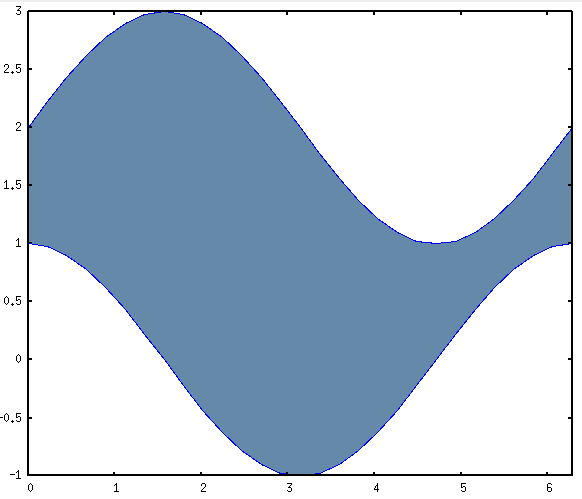
\includegraphics[width=6cm]{images/04_analisis2/region_tipo_1.png}
\end{center}

Esta región $R$ es una región elemental tipo I. 
\end{example}

\begin{observation}
Como todas las funciones que definen una región elemental $R$ son contínuas en un compacto, resultan ser acotadas, por lo tanto $R$ es un conjunto acotado, y como $R$ es cerrado, resulta que además $R$ es compacto.
\end{observation}

\section{Teorema de Fubini en $\RR^2$}

El siguiente teorema nos permite calcular ciertas integrales dobles realizando dos integrales simples iteradas.

\begin{theorem}[Fubini] \index{Integral múltiple!Teo. Fubini}
Sea $f : A \subset \RR^2 \to \RR$ contínua, con $ A$ región elemental tipo I, de la forma $A = \{(x,y) \in \RR^2 : a \leq x \leq b, f(x) \leq y \leq g(x) \}$ entonces

$$ \iint_A f(x,y) dxdy = \int_a^b dx \int_{f(x)}^{g(x)} f(x,y) dy $$
\end{theorem}

\begin{observation}
Si $A$ es una región elemental tipo I y II, entonces puedo cambiar el orden de integración.
\end{observation}

\section{Teorema de cambio de variables}

Primero lo enunciamos en $\RR^2$

\begin{theorem}[Cambio variables] \index{Integral múltiple!Cambio de variables}
Sea $f : A \subset \RR^2 \to \RR$ contínua, y $g : U \subseteq \RR^2 \to \RR^2$ biyectiva, $g \in C^1$, y $(x,y) = g(u,v)$, y sea $ A = g(B)$, entonces

$$ \displaystyle \iint_{A=g(B)} f(x,y) dxdy = \iint_{B} f(g(u,v)) ||det(Dg(u,v))|| dudv $$
\end{theorem}

Ahora enunciamos la versión del teorema para $\RR^3$

\begin{theorem}
Sea $f : A \subset \RR^3 \to \RR$ contínua, y $g : U \subseteq \RR^3 \to \RR^3$ biyectiva, $g \in C^1$, y $(x,y,z) = g(u,v,w)$, y sea $ A = g(B)$, entonces

$$ \displaystyle \iiint_{A=g(B)} f(x,y,z) dxdydz = \iiint_{B} f(g(u,v,w)) ||det(Dg(u,v,w))|| dudvdw $$

\end{theorem}

\section{Coordenadas cartesianas y polares en $\RR^2$}

Son los cambios de variables más utilizados en $\RR^2$

\begin{definition}[Cartesianas]
Las \textbf{coordenadas cartesianas} corresponde a la función identidad de $\RR^2$

\begin{eqnarray*} g: \RR^2 &\to& \RR^2 \\
 g(u,v) &=& (u,v) \end{eqnarray*}

En este caso se tiene

$$ |det(Dg)| = 1 $$

Las líneas coordenadas son rectas paralelas a los ejes cartesianos.

\begin{center}
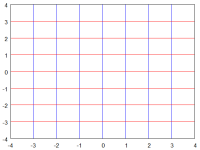
\includegraphics{images/04_analisis2/coord_cart2d.png}
\end{center}
\end{definition}

\begin{definition}[Polares] \index{Integral múltiple!Cambio de variables!Polares}
Las \textbf{coordenadas polares} corresponde al campo vectorial

\begin{eqnarray*} g : [0, +\infty) \times [0, 2\pi) &\to& \RR^2 \\
 g(\rho, \phi) &=& ( \rho \cos(\phi), \rho \sin(\phi) ) \end{eqnarray*}

En este caso se tiene

$$ |det(Dg)| = \rho $$

Las líneas coordenadas son circunferencias con centro en el origen, y semirectas que parten del origen.

\begin{center}
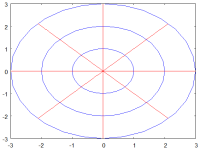
\includegraphics{images/04_analisis2/coord_polares.png}
\end{center}
\end{definition}

\section{Coordenadas cartesianas, cilíndricas y esféricas en $\RR^3$}

Son los cambios de variables más utilizados en $\RR^3$

\begin{definition}[Cartesianas]
Las \textbf{coordenadas cartesianas} corresponde a tomar la función identidad de $\RR^3$

\begin{eqnarray*} g: \RR^3 &\to& \RR^3 \\
g(u,v,w) &=& (u,v,w) \end{eqnarray*}

En este caso se tiene

$$ |det(Dg)| = 1$$

Las superficies coordenadas son planos paralelos a los planos coordenados.

\begin{center}
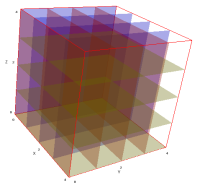
\includegraphics{images/04_analisis2/coord_cart3d.png}
\end{center}
\end{definition}

\begin{definition}[Cilíndricas] \index{Integral múltiple!Cambio de variables!Cilíndricas}
Las \textbf{coordenadas cilíndricas} sobre el eje $z$ corresponde a la función

\begin{eqnarray*} g : [0, +\infty) \times [0, 2\pi) \times \RR &\to& \RR^3 \\
g(\rho, \phi, z) &=& ( \rho \cos(\phi), \rho \sin(\phi), z ) \end{eqnarray*}

En este caso se tiene

$$ |det(Dg)| = \rho $$

Las superficies coordenadas son cilindros sobre el eje $z$, semiplanos que parten del eje $z$, y planos paralelos al $xy$.

\begin{center}
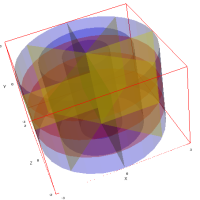
\includegraphics{images/04_analisis2/coord_cilind.png}
\end{center}
\end{definition}

\begin{example}
Calcular el volúmen del cuerpo $H$ definido como

$$ H = \begin{cases} x^2 + y^2 \leq 1 \\ 0 \leq z \leq \sqrt{x^2 + y^2} \end{cases} $$

A continuación representamos gráficamente el cuerpo $H$.  Observar que son los puntos dentro de un cilíndro de radio 1 sobre el eje $z$, y entre el plano $z=0$ y el cono $z = \sqrt{x^2 + y^2}$

\begin{center}
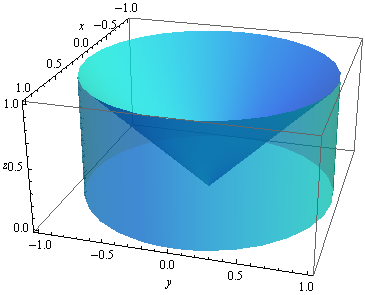
\includegraphics[width=5cm]{images/04_analisis2/tp10_ej5f.png}
\end{center}

Calculamos su volúmen

$$ Vol(H) = \iiint_H dV = \int_0^{2\pi} d\phi \int_0^1 \rho d\rho \int_0^{\rho} dz = \frac{2}{3} \pi$$
\end{example}

\begin{definition}[Esféricas] \index{Integral múltiple!Cambio de variables!Esféricas}
Las \textbf{coordenadas esféricas} sobre el eje $z$ corresponde a la función

\begin{eqnarray*} g : [0, +\infty) \times [0, 2\pi) \times [0, \pi] &\to& \RR^3 \\
g(\rho, \alpha, \beta) &=& ( \rho \cos(\alpha) \sin(\beta), \rho \sin(\alpha) \sin(\beta), \rho \cos(\beta) ) \end{eqnarray*}

En este caso

$$ |det(Dg)| = \rho^2 \sin(\beta) $$

Las superficies coordenadas son esferas centradas en el origen, conos centrados en el origen sobre el eje $z$, y semiplanos que parten del eje $z$.

\begin{center}
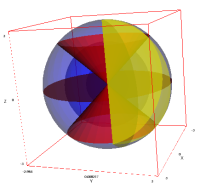
\includegraphics{images/04_analisis2/coord_esfer.png}
\end{center}
\end{definition}

\section{Ejemplos}

\begin{example}
Sea $R = \{(x,y,z) : 1 \leq x \leq 2, 1 \leq y \leq 3, 1 \leq z \leq 2 \}$ un sólido cuya densidad en cada punto es igual a la distancia del punto al plano $xy$ en gramos por $cm^3$.

Si tiro el sólido $R$ en un lago, ¿va a hundirse o va a flotar?
\end{example}

El siguiente gráfico muestra el cuerpo $R$, en rojo los puntos de mayor densidad, y en azul los de menor densidad.

\begin{center}
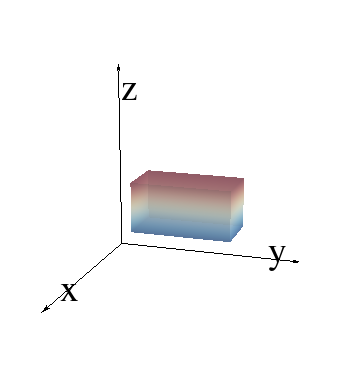
\includegraphics[scale=0.7]{images/04_analisis2/multiples3.png}
\end{center}

Recordemos que un $cm^3$ de agua pesa un gramo, es decir la densidad del agua es de $1 \ g/cm^3$.

Un litro es el volúmen ocupado por $1 \ kg$ de agua, es decir 1000 gramos, o sea un litro son $1000 \ cm^3$

El principio de Arquímedes afirma que un cuerpo totalmente sumergido en un fluido, recibe un empuje de abajo hacia arriba igual al peso del volumen del fluido que desaloja (que es exáctamente igual al volumen del cuerpo sumergido)

La densidad de un objeto es $\rho = \frac{M}{V}$ donde $m$ es la masa y $V$ el volúmen.

Por lo tanto si la densidad de un objeto es menor que la densidad del agua, el objeto flota, si es igual, el objeto permanece en equilibrio, y si es mayor, el objeto se hunde.

Calculemos la densidad $\rho = \frac{M}{V}$ del objeto.

Si integramos la función densidad sobre la región $R$ nos va a dar la masa total del sólido 

$M = \iiint_R \delta(x,y,z) dxdydz$

Si integramos la función constante 1 sobre la región $R$ nos va a dar el volúmen total del sólido

$V = \iiint_R dxdydz$

Precisamos ambos valores $M$ y $V$.

$V = \int_1^2 dx \int_1^3 dy \int_1^2 dz = (2-1)(3-1)(2-1) = 2$

Como la densidad sobre el cuerpo es $\delta(x,y,z) = z$ se tiene 

$M = \int_1^2 dx \int_1^3 dy \int_1^2 z dz = \int_1^2 dx \int_1^3 dy \frac{1}{2} [z^2]_1^2 = \frac{3}{2} \int_1^2 dx \int_1^3 dy = 3 $

Luego la densidad del cuerpo $R$ es $\rho = \frac{3}{2} > 1$, es decir es mayor que la densidad del agua, por lo tanto el cuerpo se hunde en el agua.

El siguiente ejemplo es el mismo tipo de ejercicio, pero con cuentas un poco mas complicadas.

\begin{example}
La densidad de un sólido varía punto a punto según $\delta(x,y,z) = x^2 + y^2 + z^2 \ gramos/cm^3$

(Es poco denso cerca del origen, y muy denso lejos del origen)

Si un sólido $R$ tiene techo $z = 32 - x^2 - y^2$ y piso $z = x^2 + y^2 - 40$, y tiro el sólido en un lago, ¿va a hundirse o va a flotar?
\end{example}

El siguiente gráfico muestra el sólido $R$.  En color rojo están las zonas de mayor densidad, y en azul las de menor densidad.

\begin{center}
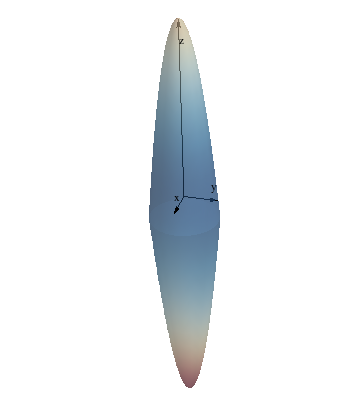
\includegraphics[scale=0.8]{images/04_analisis2/multiples2.png}
\end{center}

Calculemos la densidad $\rho = \frac{M}{V}$ del objeto.

El piso y el techo se intersectan en

$ \begin{cases} z = 32 - x^2 - y^2 \\ z = x^2 + y^2 - 40 \end{cases}$

$32-z = z + 40$

$2z = 32-40 = -8$, luego $z = -4$, y $x^2 + y^2 = 36 = 6^2 $

En coordenadas cilíndricas el cuerpo queda

$R_c = \begin{cases} 0 \leq \phi \leq 2 \pi \\ 0 \leq \rho \leq 6 \\ \rho^2 - 40 \leq z \leq 32 - \rho^2 \end{cases}$

Recordando que el jacobiano es $\rho$, nos queda

$V = \int_0^{2\pi} d\phi \int_0^6 \rho d\rho \int_{\rho^2 - 40}^{32-\rho^2} dz $

$ = \int_0^{2\pi} d\phi \int_0^6 \rho [32 - \rho^2 - \rho^2 + 40] d\rho $

$ = \int_0^{2\pi} d\phi \int_0^6 \rho [72 - 2\rho^2] d\rho $

$ = \int_0^{2\pi} d\phi \int_0^6 72\rho - 2\rho^3 d\rho $

$ = \int_0^{2\pi} d\phi [36 \rho^2 - \frac{1}{2} \rho^4]_0^6 $

$ = (1296-648) \int_0^{2\pi} d\phi $

$ = 648 \cdot 2 \pi = \boxed{1296 \pi}$

La densidad de masa en cilíndricas es $\rho^2 + z^2$, luego

$M = \int_0^{2\pi} d\phi \int_0^6 \rho d\rho \int_{\rho^2 - 40}^{32-\rho^2} (\rho^2 + z^2) dz $

$ = \int_0^{2\pi} d\phi \int_0^6 \rho^3 d\rho \int_{\rho^2 - 40}^{32-\rho^2} dz + \int_0^{2\pi} d\phi \int_0^6 \rho d\rho \int_{\rho^2 - 40}^{32-\rho^2} z^2 dz $

Resolviendo ambas integrales queda

$ = 15552 \pi + 300672 \pi = \boxed{316224 \pi}$

Luego la densidad del cuerpo es

$\rho = \frac{M}{V} = \frac{316224}{1296} = 244 \ g/cm^3 > 1 \ g/cm^3$

Como la densidad del cuerpo es mayor que la del agua, el cuerpo se hunde.

El siguiente ejemplo nos muestra que a veces es más fácil escribir la transformación inversa a la que precisamos, pero salvo por un abuso de notación a veces también es sencillo resolver una integral de esa manera.

\begin{example}
Sea $R$ la región limitada por $y = x$, $y = x+1$, $xy=1$, $xy=3$, en el primer cuadrante.

Calcular $\iint_{R} 2x+2y \ dxdy$
\end{example}

Sería complicado calcularlo en el plano $xy$.  A continuación está el gráfico de la región $R$ en el plano $xy$.

\begin{center}
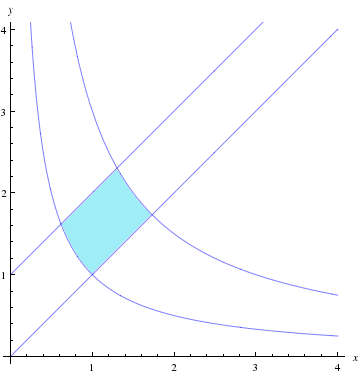
\includegraphics[scale=0.7]{images/04_analisis2/multiples.png}
\end{center}

Conviene pasar a un plano $uv$, pero en este caso resulta más sencillo escribir el cambio de variables desde $xy$ hasta $uv$.  

Proponemos el cambio de variables

$(u,v) = h(x,y) = (y-x, xy)$

Calculemos el jacobiano 

$Dh = \begin{pmatrix} -1 & 1 \\ y & x \end{pmatrix}$

y su determinante

$det(Dh) = -x - y$

en valor absuluto

$|det(Dh)| = x+y$

El problema que tenemos es que para aplicar el teorema de cambio de variables, la transformación debería ir de $uv$ a $xy$, es decir que precisamos el cambio de variables inverso $g = h^{-1}$.  Pero entonces se tiene (con un abuso de notación) que $|det(Dg)| = |det(Dh^{-1})| = |det(Dh)|^{-1} = \frac{1}{x+y}$.

Notar que la región $R$ del plano $xy$ se transforma en la región $U$ rectangular del plano $uv$ con $U = \{(u,v) : 0 \leq u \leq 1, 1 \leq v \leq 3 \}$

Por lo tanto (de nuevo con un abuso de notación)

$\iint_{R} 2x+2y \ dxdy = \iint_U (2x+2y) \frac{1}{x+y} dudv$

$= 2 \iint_U dudv = 2 Area(U) = 2 \cdot (1-0) \cdot (3-1) = 4$


% % % % % % % % % % % % % % % % % % % % % % % % % % % % % %

\chapter{Integrales de Superficie y Flujo}

\section{Definición para superficie paramétrica}

\begin{definition}[Integral superficie] \index{Integral de superficie}
Dada una superficie $\Sigma \in \RR^3$ con parametrización $ g: B \subseteq \RR^2 \to \RR^3$, y dado un campo escalar $f : A \subseteq \RR^3 \to \RR$ contínuo, tal que $\Sigma \in A^{\circ}$, definimos el diferencial de superficie escalar como

$$ ds = || g'_u(u,v) \wedge g'_v(u,v) || dudv $$

y la integral de $f$ sobre $\Sigma$ como

$$ \iint_\Sigma f ds = \iint_B f(g(u,v)) || g'_u(u,v) \wedge g'_v(u,v) || dudv $$

Definimos el área de la superficie $\Sigma$ como la integral de la función constante 1, es decir

$$ area(\Sigma) = \iint_{\Sigma} ds = \iint_B || g'_u(u,v) \wedge g'_v(u,v) || dudv $$

Dada la misma superficie $\Sigma$ (orientable) con misma parametrización $g$, y dado el campo vectorial $f : A \subseteq \RR^3 \to \RR^3$ contínuo, tal que $\Sigma \in A^{\circ}$, definimos el diferencial de superficie vectorial como

$$ ds = ( g'_u(u,v) \wedge g'_v(u,v) ) dudv $$

y definimos la integral de $f$ sobre $\Sigma$ en este caso también llamado \textbf{flujo} como \index{Integral de superficie!Flujo}

$$ \iint_\Sigma f \cdot ds = \iint_B f(g(u,v)) \cdot (g'_u(u,v) \wedge g'_v(u,v)) dudv $$

En este caso decimos que se trata de la integral sobre la superficie $\Sigma$ en la orientación con vector normal $g'_u(u,v) \wedge g'_v(u,v)$.
\end{definition}

\section{Caso superficie gráfica de campo escalar}

Sea $f: A \subset \RR^2 \to \RR$, su conjunto gráfica consiste en el conjunto 

$$ \Sigma = \{(x,y,z) \in A \times \RR : z = f(x,y)\}$$

La misma la podemos parametrizar como 

$$ g(x,y) = (x,y, h(x,y)) $$

Luego

\begin{eqnarray*} g'_x &=& (1,0,h'_x) \\
g'_y &=& (0,1,h'_y) \\
g'_x \wedge g'_y &=& (-f'_x, -f'_y, 1) \end{eqnarray*}

Por lo tanto, el diferencial de superficie vectorial es

$$ ds = (-f'_x, -f'_y, 1)dxdy $$

y el diferencial de superficie escalar es

$$ ds = \sqrt{1 + (f'_x)^2 + (f'_y)^2 }dxdy $$

\section{Caso superficie definida implícitamente}

Sea el campo escalar $ G: A \subset \RR^3 \to \RR$, $ G \in C^1$ y supongamos la superficie $\Sigma$ corresponde al conjunto de nivel 0 de $G$.  Es decir es la superficie de ecuación 

$$G(x,y,z) = 0$$ 

y supongamos además que $G'_z(x,y,z) \neq 0$

Entonces por el teorema \ref{cauchy_dini} de Cauchy-Dini, la ecuación define implícitamente a $z = w(x,y)$, con $w$ diferenciable.  Luego podemos parametrizar $\Sigma$ de la siguiente forma

$$ g(x,y) = (x,y, w(x,y) )$$

\begin{eqnarray*} g'_x &=& (1,0, w'_x) \\
g'_y &=& (0,1, w'_y) \\
g'_x \wedge g'_y &=& (-w'_x, -w'_y, 1) \end{eqnarray*}

Pero

\begin{eqnarray*} w'_x &=& - \frac{G'_x}{G'_z} \\
w'_y &=& - \frac{G'_y}{G'_z} \end{eqnarray*}

reemplazando

$$ g'_x \wedge g'_y = (\frac{G'_x}{G'_z}, \frac{G'_x}{G'_z}, 1) = \frac{1}{G'_z}\nabla G$$

Por lo tanto, el diferencial de superficie vectorial es

$$ ds = \frac{\nabla G}{G'_z}dxdy $$

y el diferencial de superficie escalar es

$$ ds = \frac{||\nabla G||}{|G'_z|}dxdy $$


% % % % % % % % % % % % % % % % % % % % % % % % % % % % % %

\chapter{Cálculo de Masa, momentos, y centro}

\section{Valor medio de una función}

Dada una función $f(x)$ definida en un intervalo $a \leq x \leq b$, el valor medio de $f(x)$ en dicho intervalo es

$$ \frac{1}{b-a} \int_a^b f(x) dx $$

Si uno toma $n$ valores $f(x_1), f(x_2), \ldots, f(x_n)$ y calcula su promedio $\frac{1}{n} \sum_{i=1}^n f(x_i)$ para $n$ grande se aproxima mucho al valor medio de una función.

La explicación de este fenómeno se debe a que la altura de un rectánculo de base $a \leq x \leq b$ tal que tiene el mismo área bajo la curva que $f$ es precisamente $ \frac{1}{b-a} \int_a^b f(x) dx$

Pues si llamamos $h$ a dicha altura

$(b-a) h = \int_a^b f(x) dx$

de donde $ h = \frac{1}{b-a} \int_a^b f(x) dx$

Similarmente para integrales dobles, el valor medio de una función $f(x,y)$ es

$$ \frac{\iint_R f(x,y) dxdy}{ \iint_R dxdy }$$

Más generalmente, si $R$ es una región (curva, plana, o sólida) y llamamos $dv$ al diferencial (de curva, área o volumen) y $f$ una función contínua definida sobre $R$, entonces el valor medio de $f$ en $R$ es

$$ \frac{ \int_R f dv }{ \int_R dv }  $$

\section{Valor medio con peso}

Dada una función no negativa $p(x,y,z)$, la pensamos como una función peso, es decir cuanto más grande sea $p(x,y,z)$ mayor es el peso del punto $(x,y,z)$.

El valor medio con peso de una función $f(x,y,z)$ respecto al peso $p(x,y,z)$ en una región $R$ en el espacio es el número

$$\frac{ \iiint_R f(x,y,z) p(x,y,z) dxdydz}{ \iiint_R p(x,y,z) dxdydz} $$

Más generalmente, si $R$ es una región (curva, plana, o sólida) y llamamos $dv$ al diferencial (de curva, área o volumen) y $f$ una función contínua definida sobre $R$, entonces el valor medio de $f$ con peso $p$ en $R$ es

$$\frac{ \int_R f \cdot p \ dv}{ \int_R p \ dv} $$

\section{Centro de masa}

Dado un sólido $R$ tiene densidad $p(x,y,z)$ en cada punto $(x,y,z)$

El centro de masa es $(x_\mu, y_\mu, z_\mu)$

donde

$x_\mu =$ el valor medio de $f(x,y,z) = x$ respecto a $p(x,y,z)$ en $R$

$y_\mu =$ el valor medio de $f(x,y,z) = y$ respecto a $p(x,y,z)$ en $R$

$z_\mu =$ el valor medio de $f(x,y,z) = z$ respecto a $p(x,y,z)$ en $R$

Más generalmente, si $R$ es una región (curva, plana, o sólida) en $\RR^n$ y llamamos $dv$ al diferencial (de curva, área o volumen) y $p$ es la densidad de masa en cada punto, entonces el centro de masa es $(x_{i_\mu})_{1 \leq i \leq n} $

donde $x_{i_\mu}$ es el valor medio de $f=x_i$ respecto de $p$ en $R$.

\section{Fórmulas}

Veamos algunas fórmulas para el cálculo de masa, momentos y centro, sobre curvas y regiones planas.

Sea $ C \subset \RR^2$ una curva, y $A \subseteq \RR^2$ una región plana.

Sea $ \delta: \RR^2 \to \RR$ contínua la densidad de masa.

\begin{center}
\begin{tabular}{|p{4cm}|c|c| }
  \hline
  Concepto                               & Curvas                       & Región plana                    \\
  \hline
  \hline
  $M$: Masa                                   & $\int_C \delta dc$       & $\iint_A \delta dxdy$       \\
  \hline
  $M_x$: Momento estático respecto al eje $x$   & $\int_C y \delta dc$   & $\iint_A y \delta dxdy$   \\
  \hline
  $M_y$: Momento estático respecto al eje $y$   & $\int_C x \delta dc$   & $\iint_A x \delta dxdy$   \\
  \hline
  $G$: Centro de masa                         & $ \frac{1}{M} (M_y, M_x)$ & $ \frac{1}{M} (M_y, M_x)$    \\
  \hline
  $I_x$: Momento de inercia respecto al eje $x$ & $ \int_C y^2 \delta dc$ & $\iint_A y^2 \delta dxdy$ \\
  \hline
  $I_y$: Momento de inercia respecto al eje $y$ & $ \int_C x^2 \delta dc$ & $ \iint_A x^2 \delta dxdy$ \\
  \hline

\end{tabular}
\end{center}


Ahora en $\RR^3$.  Veamos algunas fórmulas para el cálculo de masa, momentos y centro, sobre curvas en el espacio, regiones sólidas, y supercicies.

Sea $ C \subset \RR^3$ una curva, $A \subseteq \RR^3$ una región sólida, y $\Sigma \subseteq \RR^3$ una superficie.

Sea $ \delta: \RR^3 \to \RR$ contínua la densidad de masa.

\onecolumn

\begin{center}
\begin{tabular}{|p{4cm}|c|c|c| }
  \hline
  Concepto                                  & Curvas                        & Región sólida                       & Superficie\\
  \hline
  \hline
  $M$: Masa                                  & $\int_C \delta dc$        & $\iiint_A \delta dxdydz$        & $\iint_{\Sigma} \delta ds$ \\
  \hline
  $M_{xy}$: Momento estático respecto al plano $xy$  & $\int_C z \delta dc$ & $\iiint_A z \delta dxdydz$ & $\iint_{\Sigma} z \delta ds$ \\
  \hline
  $M_{xz}$: Momento estático respecto al plano $xz$  & $\int_C y \delta dc$ & $\iiint_A y \delta dxdydz$ & $\iint_{\Sigma} y \delta ds$ \\
  \hline
  $M_{yz}$: Momento estático respecto al plano $yz$   & $\int_C x \delta dc$ & $\iiint_A x \delta dxdydz$ & $\iint_{\Sigma} x \delta ds$ \\
  \hline
  $G$: Centro de masa                            & $\frac{1}{M} (M_{yz}, M_{xz}, M_{xy})$  & $\frac{1}{M} (M_{yz}, M_{xz}, M_{xy})$ & $\frac{1}{M} (M_{yz}, M_{xz}, M_{xy})$ \\
  \hline
  $M_x$: Momento estático respecto al eje $x$     & $\int_C \sqrt{y^2 + z^2} \delta dc$  & $\iiint_A \sqrt{y^2 + z^2} \delta dxdydz$ & $\iint_{\Sigma} \sqrt{y^2 + z^2} \delta ds$ \\
  \hline
  $M_y$: Momento estático respecto al eje $y$     & $\int_C \sqrt{x^2 + z^2} \delta dc$  & $\iiint_A \sqrt{x^2 + z^2} \delta dxdydz$ & $\iint_{\Sigma} \sqrt{x^2 + z^2} \delta ds$ \\
  \hline
  $M_z$: Momento estático respecto al eje $z$     & $\int_C \sqrt{x^2 + y^2} \delta dc$  & $\iiint_A \sqrt{x^2 + y^2} \delta dxdydz$ & $\iint_{\Sigma} \sqrt{x^2 + y^2} \delta ds$ \\
  \hline
  $I_{xy}$: Momento de inercia respecto al plano $xy$ & $\int_C z^2 \delta dc$ & $ \iiint_A z^2 \delta dxdydz$ & $\iint_{\Sigma} z^2 \delta ds$ \\
  \hline
  $I_{xz}$: Momento de inercia respecto al plano $xz$ & $\int_C y^2 \delta dc$ & $ \iiint_A y^2 \delta dxdydz$ & $\iint_{\Sigma} y^2 \delta ds$ \\
  \hline
  $I_{yz}$: Momento de inercia respecto al plano $yz$ & $\int_C x^2 \delta dc$ & $ \iiint_A x^2 \delta dxdydz$ & $\iint_{\Sigma} x^2 \delta ds$ \\
  \hline
  $I_{x}$: Momento de inercia respecto al eje $x$ & $\int_C (y^2 + z^2) \delta dc$ & $ \iiint_A (y^2 + z^2) \delta dxdydz$ & $\iint_{\Sigma} (y^2+z^2) \delta ds$ \\
  \hline
  $I_{y}$: Momento de inercia respecto al eje $y$ & $\int_C (x^2 + z^2) \delta dc$ & $ \iiint_A (x^2 + z^2) \delta dxdydz$ & $\iint_{\Sigma} (x^2+z^2) \delta ds$ \\
  \hline
  $I_{z}$: Momento de inercia respecto al eje $z$ & $\int_C (x^2 + y^2) \delta dc$ & $ \iiint_A (x^2 + y^2) \delta dxdydz$ & $\iint_{\Sigma} (x^2+y^2) \delta ds$ \\
  \hline

\end{tabular}
\end{center}

Más generalmente: 

El \textbf{momento estático} respecto a una recta (o plano) es la integral de la distancia a la recta (o plano) por la densidad de masa. 
 
El \textbf{momento de inercia} respecto a una recta (o plano) es la integral de la distancia al cuadrado a la recta (o plano) por la densiad de masa.


% % % % % % % % % % % % % % % % % % % % % % % % % % % % % %

\chapter{Teoremas de Green, Stokes y Gauss}

\begin{definition}
Sea $f : A \subset \RR^2 \to \RR^2$, $f \in C^1$,  $ f=(P,Q)$, entonces definimos el green de $f$ como

$$ green(f) = Q'_x - P'_y $$

El \textbf{operador nabla} corresponde a $ \nabla = \left( \frac{\partial}{\partial x}, \frac{\partial}{\partial y}, \frac{\partial}{\partial z} \right)$.

Sea $f : A \subset \RR^3 \to \RR^3$, $f \in C^1$, $ f=(P,Q,R)$, entonces definimos el rotor de $f$ como

$$ rot(f) = \nabla \wedge f = (R'_y - Q'_z, P'_z - R'_x, Q'_x - P'_y) $$

y la divergencia de $f$ como

$$ div(f) = \nabla \cdot f = P'_x + Q'_y + R'_z $$
\end{definition}

\begin{theorem}[Teorema de Green] \index{Teoremas integrales!Green}
Dada una región elemental $ A \subset \RR^2$ con curva frontera $ C = \partial A$ regular o regular a trozos (automáticamente cerrada y simple, o sea de Jordan), y sea el campo vectorial $f : B \subset \RR^2 \to \RR^2$, $f \in C^1$, $f = (P,Q)$, y con $ A \subset B$, entonces

$$ \displaystyle \oint_{C^+ = \partial A} f \cdot dc = \iint_A Q'_x - P'_y dxdy $$
\end{theorem}

\begin{theorem}[Teorema de Stokes] \index{Teoremas integrales!Stokes}
Dada una superficie (orientable) abierta $ \Sigma \subset \RR^3$ y su curva borde $ C = \partial \Sigma$ regular/a trozos (automáticamente cerrada y simple), y sea $ f : A \subset \RR^3 \to \RR^3$, $f \in C^1$ con $ f = (P,Q,R)$, y con $ \Sigma \subset A$, entonces

$$ \displaystyle \oint_{C^+ = \partial \Sigma} f \cdot dc = \iint_{\Sigma} rot(f) \cdot ds $$
\end{theorem}

\begin{theorem}[Teorema de la divergencia] \index{Teoremas integrales!Gauss}
Dada una región elemental del espacio $H \subset \RR^3$, y su superficie frontera $ \Sigma = \partial H$ una superficie regular/a trozos (automáticamente cerrada y simple), y sea $ f : A \subset \RR^3 \to \RR^3$, $f \in C^1$, con $ f = (P,Q,R)$, y $ H \subset A$, entonces

$$ \displaystyle \iint_{\Sigma^+ = \partial H} f \cdot ds = \iiint_H div(f) dxdydz $$
\end{theorem}

\section{Campos irrotacionales, solenoidales, y armónicos}

\begin{definition}
Sea $A \subset \RR^n$ un conjunto abierto.

Un campo vectorial $f: A \subset \RR^3 \to \RR^3$, $ f \in C^1$ se dice \textbf{irrotacional} \index{Teoremas integrales!Irrotacional} si $ rot(f) = 0$

Un campo vectorial $f: A \subset \RR^3 \to \RR^3$, $ f \in C^1$ se dice \textbf{solenoidal} \index{Teoremas integrales!Solenoidal} si $ div(f) = 0$

Un campo escalar $ f: A \subset \RR^3 \to \RR$, $ f \in C^1$ se dice \textbf{armónico} \index{Teoremas integrales!Armónico} si $ div(grad(f)) = 0$
\end{definition}

\begin{theorem}
Sea el campo escalar $f: A \subset \RR^3 \to \RR$, $ f \in C^2$, entonces $ rot(grad(f)) = 0$, es decir los campos de gradientes son irrotacionales.

Sea el campo vectorial $f: A \subset \RR^3 \to \RR^3$ con $ f \in C^2$, entonces $div(rot(f)) = 0$, es decir los campos de rotores son solenoidales.
\end{theorem}


\section{Green para cálculo de área}

El teorema de Green puede aplicarse para calcular áreas de regiones planas.  Para ello elegimos alguna función $f : \RR^2 \to \RR^2$, $f = (P,Q)$ tal que $Q'_x - P'_y = k$ sea constante no nula.  En ese caso si $A \subseteq \RR^2$ es una región elemental con curva frontera $C = \partial $ regular/a trozos, entonces por el teorema de Green

$$ \oint_C f \ dc = \iint_A Q'_x - P'_y dxdy = k \iint_A dxdy $$

de donde

$$ Area(A) = \frac{1}{k} \oint_c f \ dc $$

\section{Green para región múltiplemente conexa}

Si $R = A - \bigcup_{i=1}^n A_i $ con $A$ y $A_i$ símplemente conexos para todo $1 \leq i \leq n$, y los $A_i$ disjuntos dos a dos, y con frontera $C_a = \partial A$ y $C_i = \partial A_i$ regular/a trozos, y $C = \partial R$

Sea $f : R \subseteq \RR^2 \to \RR^2$, $f(x,y) = (P(x,y), Q(x,y)) \in C^1 $

Entonces

$$ \iint_R Q'_x - P'_y dxdy = \int_{C_a} f dc - \sum_{i=1}^n \int_{C_i} f dc = \int_C f dc $$

es decir

$$\int_C f dc = \int_{C_a} f dc - \sum_{i=1}^n \int_{C_i} f dc $$

y en particular si $Q'_x - P'_y = 0$ entonces

$$ \int_{C_a} f dc = \sum_{i=1}^n \int_{C_i} f dc $$

más en particular, si además $n=1$ se tiene

$$ \int_{C_a} f dc = \int_{C_1} f dc $$

es decir que la circulación sólo depende de si se encierra a $C_1$ o no.  Si no lo encierra el interior es símplemente conexo y por Green y la circulación da cero.  Si lo encierra por Green da lo mismo que la circulación sobre $C_1$.  Si la curva $C_1$ la reducimos a un punto, la circulación depende sólo de si encierra o no a dicho punto.

Se entiende que todas las curvas están orientadas en forma positiva, es decir $C_a$ y las $C_i$ en forma antihoraria, y la curva $C = \partial R$ que en realidad está compuesta por $C_a$ y las $C_i$ para todo $1 \leq i \leq n$, está orientada con $C_a$ en forma antihoraria y las $C_i$ en forma horaria.

\begin{example}
Sea $R = \{ (x,y) : x^2 + y^2 \leq 4, (x-1)^2 + y^2 \geq 1/4, (x+1)^2 + y^2 \geq 1/4 \}$

\begin{itemize}
\item[a] Sea $f(x,y) = (P(x,y), Q(x,y)) \in C^1$, con $Q'_x - P'_y = 3$.

Calcule la circulación de $f$ sobre $C = \partial R$.

\item[b] Si $Q'_x - P'_y = 0$ y la circulación en forma antihoraria de $C_1$ es $3\pi$ y la circulación en forma horaria de $C_2$ es $-7 \pi$, calcular la circulación sobre $C_a$ (donde $C_a, C_1, C_2$ son las circunferencia de radio 2 y las de radio 1/2 respectivamente)

\end{itemize}

\end{example}

El siguiente gráfico muestra en color gris la región $R$.

\begin{center}
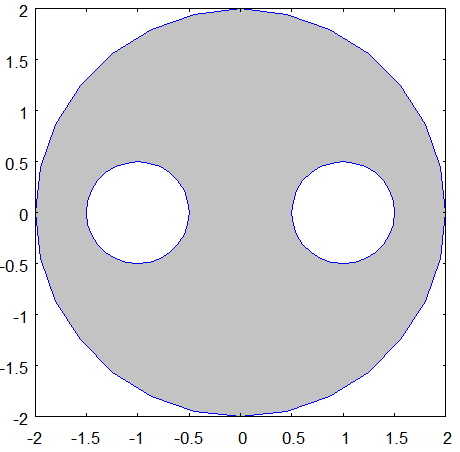
\includegraphics{images/04_analisis2/segundo_parcial_2_3_2012.png}
\end{center}

\begin{itemize}
\item[a] Aplicamos Green para región múltiplemente conexa

$ \iint_R Q'_x - P'_y dxdy = 3 Area(R) = 3 [4 \pi - (\pi/4 + \pi/4)] = \frac{21}{2} \pi = \int_C f dc$

donde $C$ se orientó con la circunferencia de radio 2 en forma antihoraria, y las circunferencias interiores en forma horaria.

\item[b] La circulación sobre $C_2$ en forma antihoraria es $-(-7\pi) = 7\pi$.  Luego como $Q'_x - P'_y = 0$ se tiene que $\int_{C_a} f dc = \int_{C_1} f dc + \int_{C_2} f dc = 3 \pi + 7\pi = 10 \pi$, donde todas las curvas están orientadas en forma antihoraria.
\end{itemize}


% % % % % % % % % % % % % % % % % % % % % % % % % % % % % %

\chapter{Ecuaciones Diferenciales 2º parte}

\section{Ecuación diferencial ordinaria homogénea}

\begin{definition}
Una función $f : A \subseteq \RR^n \to \RR^m$ se dice \textbf{homogénea de grado $k$} si 

$$F(\lambda x) = \lambda^k F(x)$$
\end{definition}

\begin{definition}[EDO homogénea] \index{Ecuación Diferencial!Homogénea}
Una ecuación diferencial ordinaria se dice homogénea si se puede expresar en la forma

$$ y' = F(x,y) $$

donde $F$ es una \textbf{función homogénea} de grado cero, es decir si $F(tx, ty) = F(x,y)$
\end{definition}

Para resolverla se hace la sustitución $y=zx$, donde $z$ depende de $x$.  Queda una ecuación diferencial de variables separables en $z$ que la resolvemos, y finalmente volvemos a reemplazar $z = \frac{y}{x}$.

Ahora con más detalle, para resolverla hacemos la sustitución

\begin{eqnarray*} y &=& zx \\
y' &=& z'x + z \end{eqnarray*}

la reemplazamos en la ecuación diferencial

$$ z'x + z = F(x,zx) $$

como $F$ es homogénea de grado 0

$$z'x + z = F(1,z)$$

restamos $z$ de ambos lados

$$z' x = F(1,z) - z$$

separo variables e integro

$$ \int \frac{dz}{F(1,z) - z} = \int \frac{dx}{x} + C$$

Esa es la solución general de $z$, para obtener la solución general de $y$ se reemplaza $z = \frac{y}{x}$ y listo.

\section{Ecuación diferencial total exacta}

\begin{definition}[Tot. exacta] \index{Ecuación Diferencial!Total exacta}
Una ecuación diferencial total exacta, es aquella que se puede expresar como

$$ P(x,y) dx + Q(x,y) dy = 0$$

con $P$ y $Q$ definidos sobre $A \subseteq \RR^2$ símplemente conexo, y tal que $Q'_x - P'_y = 0$.
\end{definition}

Para resolverla, empezamos por notar que por la condición \ref{suficiente_potencial} (suficiente para la existencia de función potencial), sabemos que $f = (P,Q)$ es conservativo, y por lo tanto existe 

$$\phi : A \subseteq \RR^2 \to \RR$$

con $\phi \in C^2$ y tal que

$$ d\phi(x,y) = P(x,y)dx + Q(x,y)dy $$

Luego la solución general es de la forma

$$ \phi(x,y) = C$$

\subsection{Convertible a exacta con factor integrante}

Supongamos que queremos resolver una ecuación diferencial de la forma

$$ P(x,y) dx + Q(x,y) dy = 0$$

con $P$ y $Q$ definidos sobre $A \subseteq \RR^2$ símplemente conexo, pero tal que $Q'_x - P'_y \neq 0$.

La ecuación diferencial no es total exacta, pero a lo mejor la podemos convertir en total exacta multiplicando la ecuación por una función $\mu$ que llamaremos \textbf{factor integrante}, que la convierta en una ecuación diferencial total exacta.  Luego la resolvemos como cualquier ecuación diferencial total exacta.

El problema ahora es como encontrar un factor integrante.  Vamos a trabajar sólo con factores integrantes que dependen de una sóla variable, o bien $x$ o bien $y$.

\begin{proposition}[Factor integrante] \index{Ecuación Diferencial!Total exacta!Factor integrante}
Si $ Q'_x - P'_y \neq 0$ pero al dividirla por $P$ o por $Q$ depende sólamente de una variable, hay un factor integrante respecto de esa variable.  

Si hay factor integrante respecto a $x$ el mismo es

$$ \mu(x) = e^{\int \frac{P'_y - Q'_x}{Q} dx} $$

Si hay factor integrante respecto a $y$ el mismo es

$$ \mu(y) = e^{\int \frac{Q'_x - P'_y}{P} dy} $$
\end{proposition}

\begin{proof}
Vamos a ver el caso de factor integrante respecto a $y$.  

Supongamos que exite $\mu(y)$ tal que al multiplicar por la ecuación diferencial la convierte en total exacta, por lo tanto

$$ \mu(y) P(x,y) dx + \mu(y) Q(x,y) dy = 0$$

es total exacta, teniendo en cuenta que $\mu$ depende sólo de $y$ tenemos

$$ \mu Q'_x - [\mu' P + \mu P'_y] = 0$$

$$ \mu Q'_x - \mu' P - \mu P'_y = 0$$

$$ \mu (Q'_x - P'_y ) = \mu' P $$

$$ \frac{\mu'}{\mu} = \frac{Q'_x - P'_y}{P} $$

Como $ \frac{Q'_x - P'_y}{P}$ depende sólo de $y$, esto es una ecuación diferencial de variables separable en $\mu$, con $\mu' = d\mu / dy$, lo resolvemos

$$ \int \frac{d\mu}{\mu} = \int \frac{Q'_x - P'_y}{P} dy $$

$$ \mu(y) = e^{\int \frac{Q'_x - P'_y}{P} dy} $$

que es el factor integrante respecto a $y$.

El caso de factor integrante respecto a $x$ es análogo.
\end{proof}

\section{Ecuación diferencial lineal de 2º orden}

Recordemos que en \ref{edo_lineal_orden_n} habíamos visto la definición de la ecuación diferencial lineal de orden $n$.  Y en \ref{resolucion_lineal_1er_orden} aprendimos a resolver la ecuación diferencial lineal de primer orden.

Ahora vamos a trabajar con las lineales de segundo orden.

\begin{definition}[Lineal de 2do orden] \index{Ecuación Diferencial!Lineal!De 2do orden}
Una ecuación diferencial se dice \textbf{lineal de segundo orden} si se la puede expresar como

$$ y'' + a(x)y' + b(x) y = g(x) $$

La misma se dice \textbf{homogénea} si $g(x)$ es la función constante cero.  

En cualquier caso, la \textbf{ecuación diferencial homogénea asociada} es

$$ y'' + a(x)y' + b(x) y = 0 $$

Si $a(x)=a$ y $b(x)=b$ son funciones constantes, nos queda

$$ y'' + ay' + by = g(x) $$

y se dice que la ecuación diferencial es \textbf{a coeficientes constantes}.

\end{definition}

Nos proponemos resolver las ecuaciones diferenciales lineales de segundo orden a coeficientes constantes.  Para ello nos va a ser de mucha ayuda la siguiente

\begin{proposition}

Dada la ecuación diferencial lineal de segundo orden a coeficientes constantes

$$ y'' + ay' + by = g(x) $$

La solución general viene dada por 

$$ y = y_h + y_p$$

donde $y_h$ es la solución general de la homogénea asociada, y $y_p$ es una solución particular.

\end{proposition}

\begin{proof}

La familia $y = y_h + y_p$ ya tiene dos constantes arbitrarias (las que provienen de $y_h$), y la ecuación diferencial es de segundo orden.  Por lo tanto si satisface la EDO entonces debe ser su SG.

Reemplazamos $y = y_h + y_p$ y veamos que satisface la ecuación diferencial.

\begin{eqnarray*} y &=& y_h + y_p \\
y' &=& y'_h + y'_p \\
y'' &=& y''_h + y''_p \end{eqnarray*}

Reemplazo en 

$$ y'' + ay' + by = g(x) $$

y obtengo

$$ (y''_h + y''_p) + a(y'_h + y'_p) + b(y_h + y_p) = g(x) $$

$$ \underbrace{y''_h + ay'_h + by_h}_{0} + \underbrace{y''_p + ay'_p + by_p}_{g(x)} = g(x) $$

Por lo tanto satisface la ecuación diferencial, y debe ser su solución general.

\end{proof}

\subsection{Resolución de la homogénea asociada}

Veamos ahora como podemos resolver la ecuación diferencial homogénea asociada, que es de la forma

$$ y'' + ay' + by = 0 $$

La solución general de la homogénea asociada resulta ser un subespacio de dimensión dos del espacio vectorial de las funciones $C^2$ de $\RR$ en $\RR$.  Por lo tanto alcanza con encontrar una base de dicho subespacio, por lo tanto si $f_1, f_2$ son soluciones particulares y $ \{f_1, f_2\}$ es LI (linealmente independiente), entonces la solución general son sus combinaciones lineales, es decir

$$ y = C_1 f_1 + C_2 f_2 $$

\begin{definition}

Dadas $f_1, f_2 : A \subseteq \RR \to \RR$, $f_1, f_2 \in C^1$.  El \textbf{wronskiano} de $f_1$ y $f_2$ es el siguiente determinante

$$ W = \left| \begin{matrix} f_1 & f_2 \\ f'_1 & f'_2 \end{matrix} \right| $$

\end{definition}

\begin{proposition}

Dadas $f_1, f_2 : A \subseteq \RR \to \RR$, $f_1, f_2 \in C^1$

Si el wronskiano de $f_1$ y $f_2$ es $ W \neq 0$ entonces $ \{f_1(x), f_2(x) \}$ es LI.

\end{proposition}

Para resolver la ecuación diferencial homogénea asociada

$$ y'' + ay' + by = 0 $$

primero proponemos como solución 

\begin{eqnarray*} y &=& e^{\alpha x} \\
y' &=& \alpha e^{\alpha x} \\ 
y'' &=& \alpha^2 e^{\alpha x} \end{eqnarray*}

ahora reemplazamos en la ecuación homogénea asociada y obtenemos

$$ \alpha^2 e^{\alpha x} + a \alpha e^{\alpha x} + b e^{\alpha x} = 0 $$

sacamos factor común $e^{\alpha x}$

$$ e^{\alpha x} [ \alpha^2 + a \alpha + b ] = 0 $$

y puesto que $e^{\alpha x} > 0$ lo dividimos y obtenemos lo que se llama la \textbf{ecuación característica}

$$ \alpha^2 + a\alpha + b = 0 $$

Al resolverla puede darse sólo uno de tres casos posibles

\begin{itemize}

\item 1º Caso: $ \alpha_1, \alpha_2$ reales y distintas.  En este caso $\{e^{\alpha_1 x}, e^{\alpha_2 x}\}$ ya es linealmente independiente, y la SG es

$$ y = c_1 e^{\alpha_1 x} + c_2 e^{\alpha_2 x} $$

\item 2º Caso: $ \alpha_1 = \alpha_2 = \alpha$ reales e iguales.  En este caso $\{e^{\alpha x}, x e^{\alpha x}\}$ resulta linealmente independiente la SG es

$$ y = c_1 e^{\alpha_1 x} + c_2 x e^{\alpha_1 x} $$

\item 3º Caso: $ \alpha_1 = r+si$, $ \alpha_2 = r-si$ complejas conjugadas.  En este caso $\{e^{\alpha_1 x}, e^{\alpha_2 x}\}$ ya es linealmente independiente.  En principio la SG es

\begin{eqnarray*} y &=& c_1 e^{\alpha_1 x} + c_2 e^{\alpha_2 x} \\
y &=& c_1 e^{(r+si) x} + c_2 e^{(r-si) x} \\
y &=& e^{rx} [ c_1 e^{six} + c_2 e^{-six} ] \end{eqnarray*}

Recordemos la Fórmula de Euler que establece que

$$ e^{is} = \cos(s) + i \sin(s) $$

reemplazando en la SG

$$ y = e^{rx} [ c_1 (\cos(sx) + i \sin(sx)) + c_2 ( \cos(-sx) + i \sin(-sx) ) ] $$

usando que $\cos(x)$ es par (es decir $\cos(x) = \cos(-x)$) y que $\sin(x)$ es impar (es decir $\sin(x) = -\sin(-x)$)

$$ y = e^{rx} [ c_1 (\cos(sx) + i \sin(sx)) + c_2 ( \cos(sx) - i \sin(sx) ) ] $$

y reagrupando

$$ y = e^{rx} [ (c_1 + c_2) \cos(sx)  + i (c_1 - c_2) \sin(sx) ] $$

Llamando $C_1 = (c_1 + c_2)$ y $C_2 = i (c_1 - c_2) $ obtenemos finalmente la SG del tercer caso

$$ y = a^{rx} [C_1 \cos(sx) + C_2 \sin(sx)]$$

\end{itemize}

\subsection{Como encontrar una solución particular}

Ahora nos faltaría aprender a encontrar una solución particular de la ecuación diferencial lineal no homogénea

$$ y'' + ay' + by = g(x) $$

El método de \textbf{coeficientes indeterminados} sirve cuando la función $g(x)$ es relativamente sencilla, que en este contexto significa combinación lineal de polinomios, exponenciales o trigonométricas.

Consiste en tratar de \emph{adivinar} la forma que debe tener la solución, proponiendo como solución una familia de funciones acorde al problema, y luego se determinan los coeficientes.

\begin{itemize}
\item Si la función es polinómica, se propone una combinación lineal de polinomios genérico, en principio del mismo grado.

Por ejemplo si $g(x) = 2x^2$, propongo $y_p = ux^2 + vx + w$

\item Si la función es exponencial, se propone una combinación lineal de exponenciales.  

Por ejemplo si $g(x) = e^{2x} + 2e^x$, propongo $y_p = ue^{2x} + ve^x$

\item Si la función es trigonométrica, se propone una combinación lineal de trigonométricas.

Por ejemplo si $g(x) = \cos(2x)$,  propongo $y_p = u\cos(2x) + v\sin(2x)$

\end{itemize}

Por ejemplo

\begin{center}
\begin{tabular}{|c|c|}
  \hline
  g(x) & propongo $y_p$ \\
  \hline
  $2x^2$ & $ux^2 + vx + w$ \\
  $e^{2x} + 2e^x$ & $ue^{2x} + ve^x$ \\
  $\cos(2x)$ & $u\cos(2x) + v\sin(2x)$ \\
  \hline
\end{tabular}
\end{center}

Se reemplazan en la EDO y se averiguan los coeficientes indeterminados $u,v,w, \ldots$.

En algunos casos puede pasar que la solución propuesta ya sea solución de la homogénea asociada, en ese caso se va a llegar a un absurdo.  En ese caso lo que se puede hacer es multiplicar por $x$ la solución propuesta y volver a intentar.  Si sigue pasando puedo multiplicar por $x^2$ y volver a intentar, y así sucesivamente.


Veamos ahora el otro método, conocido como \textbf{variación de parámetros}, para encontrar una solución particular de la ecuación diferencial lineal no homogénea

$$ y'' + ay' + by = g(x) $$

y supongamos que la solución general de la homogénea asociada es

$$ y = c_1 y_1(x) + c_2 y_2(x) $$

Este método consiste en buscar una solución particular $y$ que verifique lo siguiente

\begin{eqnarray} y &=& \lambda(x) y_1(x) + \mu(x) y_2(x) \\
y' &=& \lambda(x) y'_1(x) + \mu(x) y'_2(x) \end{eqnarray}

derivando la ecuación (1) obtenemos

$$ y' = \lambda' y_1 + \lambda y'_1 + \mu' y_2 + \mu y'_2$$

para que se cumpla la ecuación (2) pedimos

\begin{eqnarray} \lambda' y_1 + \mu' y_2 = 0 \end{eqnarray}

derivando (2)

$$ y'' = \lambda' y'_1 + \lambda y''_1 + \mu' y'_2 + \mu y''_2$$

Reemplazando en la ecuación diferencial

$$ y'' + ay' + by = g(x) $$

obtenemos

$$ \lambda' y'_1 + \lambda y''_1 + \mu' y'_2 + \mu y''_2 + a (\lambda y'_1 + \mu y'_2) + b (\lambda y_1 + \mu y_2) = g(x) $$

$$ \lambda' y'_1 + \mu' y'_2 + \lambda (\underbrace{ y''_1 + a y'_1 + b y_1}_{0}) + \mu (\underbrace{y''_2 + a y'_2 + b y_2}_{0}) = g(x) $$

lo cual impone

\begin{eqnarray} \lambda' y'_1 + \mu' y'_2 = g(x) \end{eqnarray}

juntando (3) y (4) obtenemos

\begin{eqnarray} \lambda' y_1 + \mu' y_2 &=& 0 \\
\lambda' y'_1 + \mu' y'_2 &=& g(x) \end{eqnarray}

que es un sistema de ecuaciones lineales en $\lambda'$ y $\mu'$.  

Resumiendo, estamos buscando $\lambda(x)$ y $\mu(x)$ para encontrar una solución particular de la forma

$$ y = \lambda(x) y_1(x) + \mu(x) y_2(x) $$

y para ello imponemos

$$ \begin{cases} \lambda' y_1 + \mu' y_2 = 0 \\
\lambda' y'_1 + \mu' y'_2 = g(x) \end{cases}$$

Lo resolvemos por cualquier método, por ejemplo lo escribo en forma matricial

$$ \begin{pmatrix} y_1 & y_2 \\ y'_1 & y'_2 \end{pmatrix} \begin{pmatrix} \lambda' \\ \mu' \end{pmatrix} = \begin{pmatrix} 0 \\ g(x) \end{pmatrix}$$

y lo resuelvo con la regla de Cramer

$$ \lambda' = \frac{\left| \begin{matrix} 0 & y_2 \\ g(x) & y'_2 \end{matrix} \right|}{\left| \begin{matrix} y_1 & y_2 \\ y'_1 & y'_2 \end{matrix} \right|}$$

$$ \mu' = \frac{\left| \begin{matrix} y_1 & 0 \\ y'_1 & g(x) \end{matrix} \right|}{\left| \begin{matrix} y_1 & y_2 \\ y'_1 & y'_2 \end{matrix} \right|}$$

Luego se integran ambos parámetros para encontrar una primitiva de cada una, y se reemplazan para obtener la solución particular

$$ y = \lambda(x) y_1(x) + \mu(x) y_2(x) $$

\section{Líneas de campo}

\begin{definition}[Línea de campo] \index{Ecuación Diferencial!Línea de campo}
Dado un campo vectorial $f : A \in \RR^n \to \RR^n$, $f \in C^1$, una línea de campo es una curva regular $C \subseteq A$ que admite una parametrización $g : [a,b] \to \RR^n$ tal que 

$$ g'(t) = f(g(t))$$ 

para todo $ a < t < b$
\end{definition}

\begin{observation} \label{lineas_campo_r2}
En $\RR^2$, dada $f : A \subseteq \RR^2 \to \RR^2$.

Si $C$ es una línea de campo de $f = (P,Q)$ con la parametrización $g(t) = (x(t), y(t))$, entonces debe cumplir

$$g'(t) = (x'(t), y'(t)) = (P,Q) = f(g(t))$$

en notación de Leibniz

$$ (dx,dy) = (P,Q)dt $$

y por lo tanto 

$$y' = \frac{Q}{P}$$

Otra forma de pensarlo:  las líneas de campo son las curvas que en cada punto tiene la misma pendiente que el campo $(P,Q)$ que es $\Delta y / \Delta x = Q/P$, por lo tanto satisfacen la ecuación diferencial

$$y' = \frac{Q}{P}$$

Esto quiere decir que para encontrar la familia de las líneas de campo de $f$, basta encontrar la solución general de dicha ecuación diferencial.
\end{observation}

\begin{theorem}[Línea de campo conservativo] \index{Ecuación Diferencial!Línea de campo!Conservativo}
Si $f : A \subseteq \RR^n \to \RR^n$ es un campo conservativo, y $ \phi : A \subseteq \RR^n \to \RR$ es una función potencial de $f$, es decir $\nabla \phi = f$, entonces las líneas de campo de $f$ son ortogonales a los conjuntos de nivel de $\phi$.
\end{theorem}

\begin{proof}
Consideremos el conjunto de nivel $k$ de $\phi$

$$C_k(\phi) = \{x \in A : \phi(x) = k \} $$

Sea $ C_1 \subset A$ una curva incluída en $C_k(\phi)$ parametrizada por 

$$h : [a,b] \to \RR^n$$

Sea $C_2 \subset A$ una línea de campo del campo $ f = \nabla \phi$, parametrizada por 

$$ g : [c,d] \to \RR^n$$

Supongamos que ambas curvas se cruzan en $h(t_0) = g(u_0) = x_0 \in A$

Consideremos la compuesta $w = \phi \circ h $, se tiene que

$$ w(t) = \phi(h(t)) = k $$

Como ambas son diferenciables, por el teorema de la regla de la cadena

$$ w'(t_0) = \nabla \phi(h(t_0)) \cdot h'(t_0) = 0$$

como $f = \nabla \phi$, y $h(t_0) = g(u_0)$

$$ f(g(u_0)) \cdot h'(t_0) = 0$$

Y como $ g$ es una línea de campo, $ f(g(u_0)) = g'(u_0)$, y por lo tanto

$$ g'(u_0) \cdot h'(t_0) = 0 $$

Lo que muestra que estos vectores tangentes son ortogonales.  

Tanto las líneas de campo como el conjunto de nivel eran genéricos.  Es decir que las líneas de campo de $f$ y los conjuntos de nivel de $\phi$ son ortogonales en todo punto de intersección.
\end{proof}

En $\RR^2$ tenemos el siguiente caso particular, que podemos demostrar de una forma más cartesiana.

\begin{theorem}
Sea $f : A \subseteq \RR^2 \to \RR^2$ un campo conservativo, y $\phi$ una función potencial de $f$, es decir tal que $\nabla \phi = f$.

Entonces las líneas de campo de $f$ son ortogonales a las líneas equipotenciales de $\phi$.
\end{theorem}

\begin{proof}
Por la observación \ref{lineas_campo_r2}, las líneas de campo de $f$ son la familia de curvas cuya ecuación diferencial es

% reseteo el contador de ecuaciones
\setcounter{equation}{0}

\begin{eqnarray} y' = \frac{Q}{P} \end{eqnarray}

Por otro lado, si $\phi$ es una función potencial de $f$, es decir tal que $\nabla \phi = f$, entonces las líneas equipotenciales son la familia de curvas

$$ \phi(x,y) = C $$

Buscamos su ecuación diferencial, diferenciando ambos miembros

$$ \phi'_x(x,y) dx + \phi'_y(x,y) dy = 0 $$

usando que $\nabla \phi = (\phi'_x, \phi'_y) = (P,Q)$

$$ P dx + Q dy = 0 $$

$$ Q dy = - P dx $$

o equivaléntemente su ecuación diferencial es

\begin{eqnarray} y' = - \frac{P}{Q} \end{eqnarray}

De (1) y (2) vemos que dichas familias de curvas son ortogonales.  Es decir las líneas de campo de $f$ y las líneas equipotenciales de $\phi$ son familias de curvas ortogonales.
\end{proof}
